\documentclass[10pt]{article}
\usepackage[T1]{fontenc}
\usepackage{lmodern,amsmath,amssymb,booktabs,array,graphicx,tikz,pgfplots}
\usepackage[paperwidth=190mm,paperheight=224mm,margin=10mm]{geometry}
\usepackage[hidelinks]{hyperref}
\hypersetup{pdfauthor={},pdftitle={Monochrome mathematical illustrations: semiconductor-health identifiability}}
\usetikzlibrary{arrows.meta,positioning,calc,patterns}
\pgfplotsset{compat=1.18}
\newcommand{\trans}{^{\mathsf T}}\newcommand{\R}{\mathbb R}
\newcommand{\one}{\mathbf 1}\newcommand{\zero}{\mathbf 0}
\DeclareMathOperator{\rank}{rank}\DeclareMathOperator{\range}{range}
\DeclareMathOperator{\diag}{diag}\DeclareMathOperator{\Cov}{Cov}
\DeclareMathOperator{\Var}{Var}\DeclareMathOperator{\spanop}{span}
\newcommand{\FigureNote}{Visualization code prepared with assistance from OpenAI Codex.}
\pagestyle{empty}\setlength{\parindent}{0pt}
\tikzset{
 every picture/.style={font=\fontsize{9}{11}\selectfont,>=Latex},
 every node/.style={font=\fontsize{9}{11}\selectfont,inner sep=2pt},
 head/.style={font=\fontsize{9.5}{12}\selectfont\bfseries,anchor=west},
 tinytext/.style={font=\fontsize{8}{10}\selectfont},eq/.style={align=center},
 wire/.style={draw=black,line width=.5pt},arr/.style={->,black,line width=.65pt},
 device/.style={draw,fill=white,minimum width=1.1cm,minimum height=.38cm}}
\pgfplotsset{mathaxis/.style={axis lines=left,axis line style={black,line width=.5pt},
 tick style={black},tick label style={font=\fontsize{8}{10}\selectfont},
 label style={font=\fontsize{8.5}{10}\selectfont},grid=major,
 major grid style={black!15,line width=.2pt},
 legend style={font=\fontsize{8}{10}\selectfont,draw=none,fill=white},
 every axis plot/.append style={black}}}
\newcommand{\PlateTitle}[2]{\small\textbf{Mathematical plate #1}\hfill Monochrome TikZ / PGFPlots\par
 \vspace{1.5mm}{\large\bfseries #2}\par\vspace{2mm}}
\newcommand{\PlateCaption}[1]{\par\vspace{1mm}{\fontsize{8.5}{10.5}\selectfont #1\par
 \vspace{1mm}\FigureNote\par}}

\begin{document}
\PlateTitle{1}{Conduction incidence, null directions and the observable quotient}
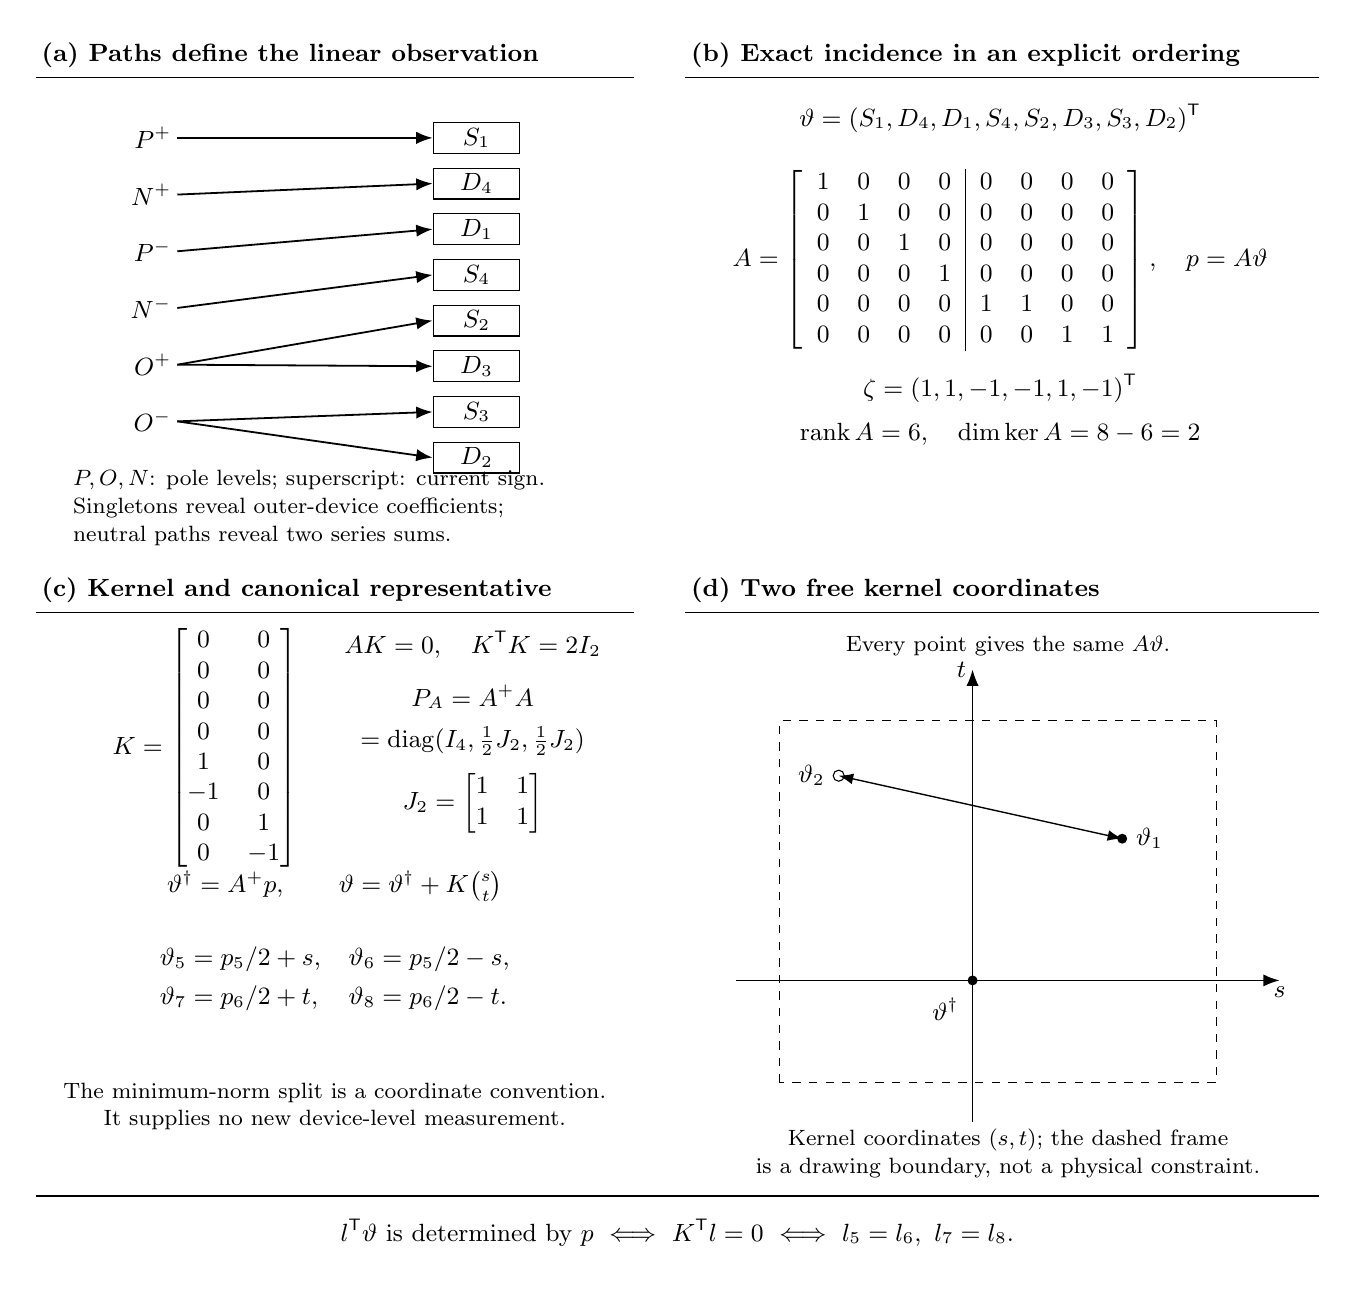
\begin{tikzpicture}[x=1cm,y=1cm]\path[use as bounding box] (0,0) rectangle (16.6,15.8);
\node[head] at (0.1,15.45){(a) Paths define the linear observation};\draw[wire] (0.1,15.17)--(7.699999999999999,15.17);
\node[head] at (8.35,15.45){(b) Exact incidence in an explicit ordering};\draw[wire] (8.35,15.17)--(16.4,15.17);
\node[anchor=east] (p0) at (1.9,14.4){$P^+$};
\node[anchor=east] (p1) at (1.9,13.68){$N^+$};
\node[anchor=east] (p2) at (1.9,12.96){$P^-$};
\node[anchor=east] (p3) at (1.9,12.24){$N^-$};
\node[anchor=east] (p4) at (1.9,11.52){$O^+$};
\node[anchor=east] (p5) at (1.9,10.8){$O^-$};
\node[device] (d0) at (5.7,14.4){$S_1$};
\node[device] (d1) at (5.7,13.82){$D_4$};
\node[device] (d2) at (5.7,13.24){$D_1$};
\node[device] (d3) at (5.7,12.66){$S_4$};
\node[device] (d4) at (5.7,12.08){$S_2$};
\node[device] (d5) at (5.7,11.5){$D_3$};
\node[device] (d6) at (5.7,10.920000000000002){$S_3$};
\node[device] (d7) at (5.7,10.34){$D_2$};
\draw[arr] (p0.east)--(d0.west);
\draw[arr] (p1.east)--(d1.west);
\draw[arr] (p2.east)--(d2.west);
\draw[arr] (p3.east)--(d3.west);
\draw[arr] (p4.east)--(d4.west);
\draw[arr] (p4.east)--(d5.west);
\draw[arr] (p5.east)--(d6.west);
\draw[arr] (p5.east)--(d7.west);
\node[tinytext,align=left,anchor=west] at (.5,9.7){$P,O,N$: pole levels; superscript: current sign.\\
Singletons reveal outer-device coefficients;\\neutral paths reveal two series sums.};
\node[eq] at (12.35,14.65){$\vartheta=(S_1,D_4,D_1,S_4,S_2,D_3,S_3,D_2)\trans$};
\node[eq] at (12.35,12.85){$A=\left[\begin{array}{cccc|cccc}
1&0&0&0&0&0&0&0\\0&1&0&0&0&0&0&0\\0&0&1&0&0&0&0&0\\0&0&0&1&0&0&0&0\\
0&0&0&0&1&1&0&0\\0&0&0&0&0&0&1&1
\end{array}\right],\quad p=A\vartheta$};
\node[eq] at (12.35,10.95){$\zeta=(1,1,-1,-1,1,-1)\trans$\\[5pt]
$\rank A=6,\quad\dim\ker A=8-6=2$};
\node[head] at (0.1,8.65){(c) Kernel and canonical representative};\draw[wire] (0.1,8.370000000000001)--(7.699999999999999,8.370000000000001);
\node[head] at (8.35,8.65){(d) Two free kernel coordinates};\draw[wire] (8.35,8.370000000000001)--(16.4,8.370000000000001);
\node[eq] at (2.25,6.65){$K=\begin{bmatrix}
0&0\\0&0\\0&0\\0&0\\1&0\\-1&0\\0&1\\0&-1\end{bmatrix}$};
\node[eq] at (5.65,6.85){$AK=0,\quad K\trans K=2I_2$\\[8pt]
$P_A=A^+A$\\[4pt]$=\diag(I_4,\tfrac12J_2,\tfrac12J_2)$\\[5pt]
$J_2=\begin{bmatrix}1&1\\1&1\end{bmatrix}$};
\node[eq] at (3.9,4.9){$\vartheta^\dagger=A^+p,\qquad\vartheta=\vartheta^\dagger+K\binom{s}{t}$};
\node[eq] at (3.9,3.72){$\begin{aligned}
\vartheta_5&=p_5/2+s,&\vartheta_6&=p_5/2-s,\\
\vartheta_7&=p_6/2+t,&\vartheta_8&=p_6/2-t.\end{aligned}$};
\node[tinytext,align=center] at (3.9,2.1){The minimum-norm split is a coordinate convention.\\It supplies no new device-level measurement.};
\draw[arr] (9.0,3.7)--(15.9,3.7) node[below] {$s$};
\draw[arr] (12.0,1.9)--(12.0,7.65) node[left] {$t$};
\draw[dashed,wire] (9.55,2.4) rectangle (15.1,7.0);
\fill (12,3.7) circle(1.8pt);\node[anchor=north east] at (11.9,3.55){$\vartheta^\dagger$};
\fill (13.9,5.5) circle(1.8pt);\node[anchor=west] at (14.0,5.5){$\vartheta_1$};
\draw[fill=white] (10.3,6.3) circle(2pt);\node[anchor=east] at (10.2,6.3){$\vartheta_2$};
\draw[<->,wire] (10.3,6.3)--(13.9,5.5);
\node[tinytext,align=center] at (12.45,7.95){Every point gives the same $A\vartheta$.};
\node[tinytext,align=center] at (12.45,1.5){Kernel coordinates $(s,t)$; the dashed frame\\is a drawing boundary, not a physical constraint.};
\draw[wire] (.1,.96)--(16.4,.96);
\node[eq] at (8.25,.5){$l\trans\vartheta\text{ is determined by }p\ \Longleftrightarrow\ K\trans l=0
\ \Longleftrightarrow\ l_5=l_6,\ l_7=l_8.$};\end{tikzpicture}
\PlateCaption{\textbf{Figure 1.} Exact T-type incidence analysis for one health channel in the ideal per-leg pole-drop observation. Device symbols in $\vartheta$ denote coefficient coordinates. The reordered columns expose the two inseparable neutral pairs. Panels (c)--(d) show the entire unrestricted inverse image, rather than a single fitted solution. The same incidence ambiguity applies separately to threshold and resistance channels; the complete three-phase current model imposes additional restrictions.}

\newpage
\PlateTitle{2}{From path ambiguity to the complete three-phase kernel}
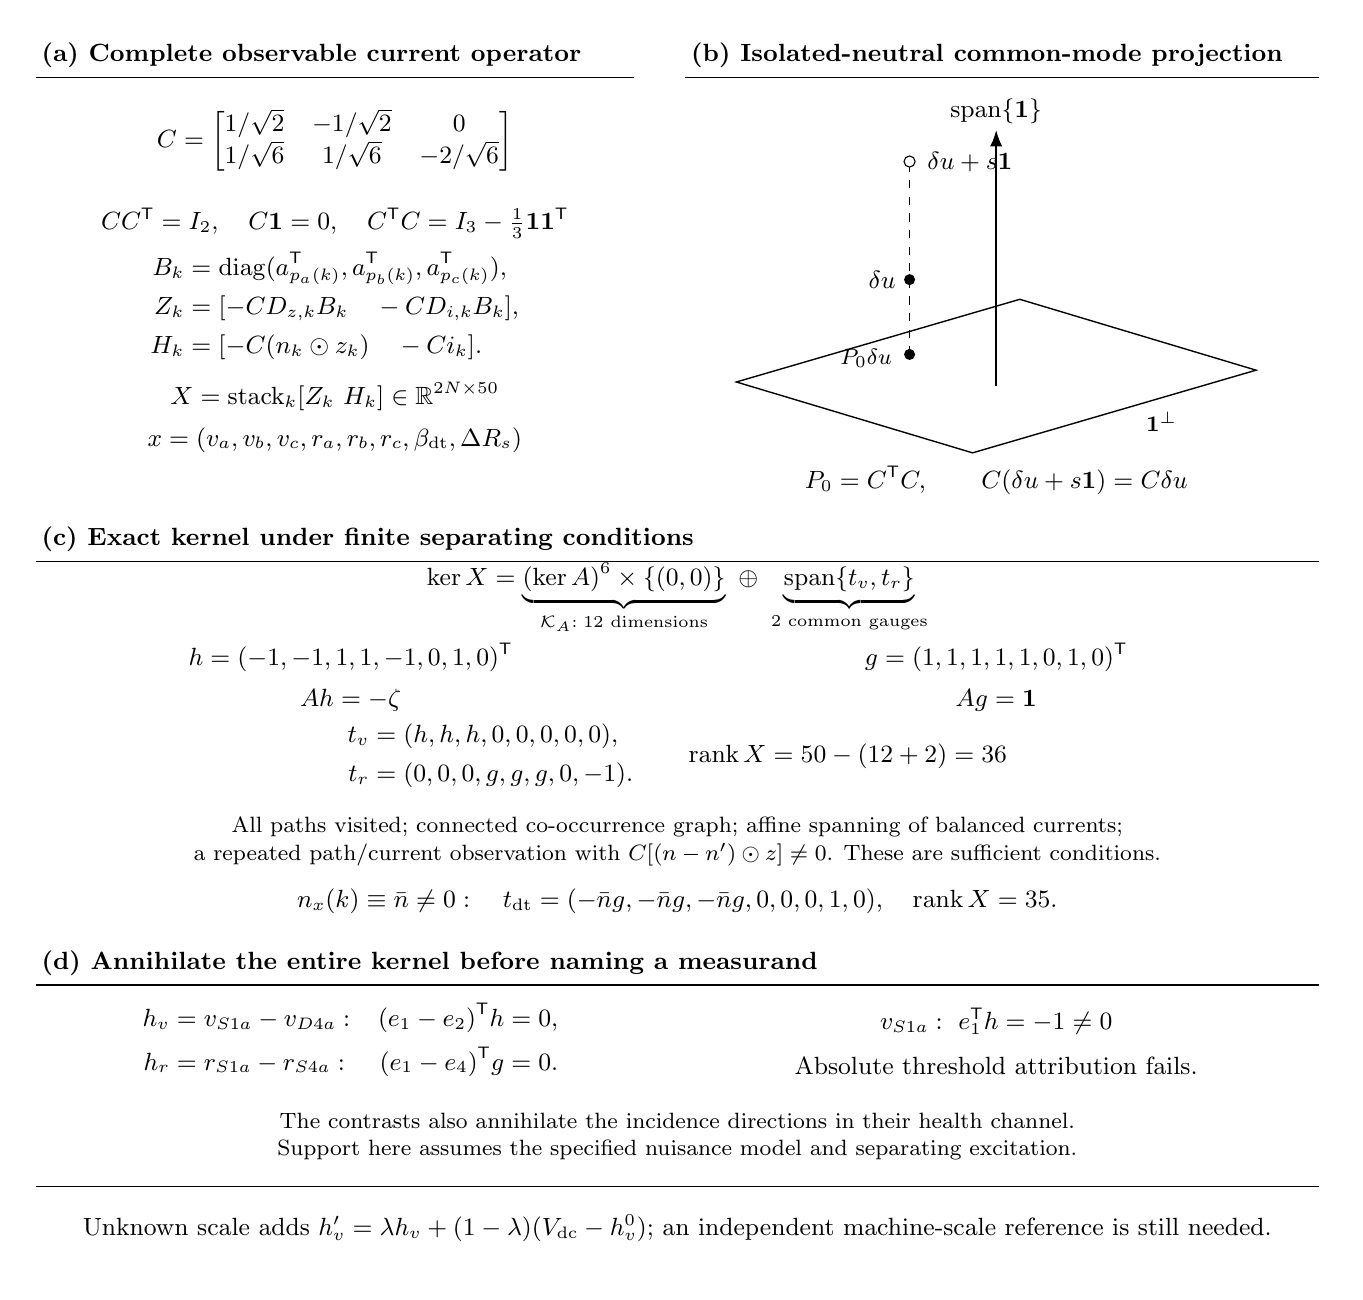
\begin{tikzpicture}[x=1cm,y=1cm]\path[use as bounding box] (0,0) rectangle (16.6,15.8);
\node[head] at (0.1,15.45){(a) Complete observable current operator};\draw[wire] (0.1,15.17)--(7.699999999999999,15.17);
\node[head] at (8.35,15.45){(b) Isolated-neutral common-mode projection};\draw[wire] (8.35,15.17)--(16.4,15.17);
\node[eq] at (3.9,14.36){$C=\begin{bmatrix}1/\sqrt2&-1/\sqrt2&0\\1/\sqrt6&1/\sqrt6&-2/\sqrt6\end{bmatrix}$};
\node[eq] at (3.9,13.32){$CC\trans=I_2,\quad C\one=0,\quad C\trans C=I_3-\tfrac13\one\one\trans$};
\node[eq] at (3.9,12.25){$\begin{aligned}B_k&=\diag(a_{p_a(k)}\trans,a_{p_b(k)}\trans,a_{p_c(k)}\trans),\\
Z_k&=[-CD_{z,k}B_k\quad-CD_{i,k}B_k],\\H_k&=[-C(n_k\odot z_k)\quad-Ci_k].\end{aligned}$};
\node[eq] at (3.9,10.85){$X=\operatorname{stack}_k[Z_k\ H_k]\in\R^{2N\times50}$\\[4pt]
$x=(v_a,v_b,v_c,r_a,r_b,r_c,\beta_{\mathrm{dt}},\Delta R_s)$};
\draw[wire] (9.0,11.3)--(12.0,10.4)--(15.6,11.45)--(12.6,12.35)--cycle;
\node[tinytext] at (14.4,10.8){$\one^\perp$};
\draw[arr] (12.3,11.25)--(12.3,14.5) node[above] {$\spanop\{\one\}$};
\draw[dashed,wire] (11.2,11.65)--(11.2,14.1);
\fill (11.2,12.6) circle(2pt);\node[anchor=east] at (11.1,12.6){$\delta u$};
\draw[fill=white] (11.2,14.1) circle(2pt);\node[anchor=west] at (11.35,14.1){$\delta u+s\one$};
\fill (11.2,11.65) circle(2pt);\node[anchor=east,tinytext] at (11.05,11.6){$P_0\delta u$};
\node[eq] at (12.3,10.05){$P_0=C\trans C,\qquad C(\delta u+s\one)=C\delta u$};
\node[head] at (0.1,9.3){(c) Exact kernel under finite separating conditions};\draw[wire] (0.1,9.020000000000001)--(16.400000000000002,9.020000000000001);
\node[eq] at (8.25,8.55){$\ker X=\underbrace{(\ker A)^6\times\{(0,0)\}}_{\mathcal K_A:\;12\text{ dimensions}}
\ \oplus\ \underbrace{\spanop\{t_v,t_r\}}_{2\text{ common gauges}}$};
\node[eq] at (4.1,7.55){$h=(-1,-1,1,1,-1,0,1,0)\trans$\\[4pt]$Ah=-\zeta$};
\node[eq] at (12.3,7.55){$g=(1,1,1,1,1,0,1,0)\trans$\\[4pt]$Ag=\one$};
\node[eq] at (8.25,6.55){$\begin{aligned}t_v&=(h,h,h,0,0,0,0,0),\\t_r&=(0,0,0,g,g,g,0,-1).
\end{aligned}\qquad\rank X=50-(12+2)=36$};
\node[tinytext,align=center] at (8.25,5.46){All paths visited; connected co-occurrence graph; affine spanning of balanced currents;\\a repeated path/current observation with $C[(n-n')\odot z]\neq0$. These are sufficient conditions.};
\node[eq] at (8.25,4.7){$n_x(k)\equiv\bar n\neq0:\quad t_{\mathrm{dt}}=(-\bar n g,-\bar n g,-\bar n g,0,0,0,1,0),\quad\rank X=35.$};
\node[head] at (0.1,3.92){(d) Annihilate the entire kernel before naming a measurand};\draw[wire] (0.1,3.6399999999999997)--(16.400000000000002,3.6399999999999997);
\node[eq] at (4.1,2.93){$\begin{aligned}
h_v&=v_{S1a}-v_{D4a}:&(e_1-e_2)\trans h&=0,\\
h_r&=r_{S1a}-r_{S4a}:&(e_1-e_4)\trans g&=0.\end{aligned}$};
\node[eq] at (12.3,2.93){$v_{S1a}:\ e_1\trans h=-1\neq0$\\[5pt]Absolute threshold attribution fails.};
\node[tinytext,align=center] at (8.25,1.72){The contrasts also annihilate the incidence directions in their health channel.\\Support here assumes the specified nuisance model and separating excitation.};
\draw[wire] (.1,1.08)--(16.4,1.08);
\node[eq] at (8.25,.55){Unknown scale adds $h_v'=\lambda h_v+(1-\lambda)(V_{\mathrm{dc}}-h_v^0)$; an independent machine-scale reference is still needed.};
\end{tikzpicture}
\PlateCaption{\textbf{Figure 2.} Common-mode and stator-resistance gauges are additional to the six incidence kernels. The vectors $h,g$ use Figure 1's ordering; substitution verifies both gauge directions exactly. Projection geometry is schematic, while the matrices and rank counts are exact. Rank 36 is conditional on the theorem's separating conditions, not guaranteed for every controller trajectory. Fixed commutation adds another null direction; unknown machine scale introduces a further model-specific equivalence.}

\newpage
\PlateTitle{3}{Nuisance projection, singular directions and target-specific uncertainty}
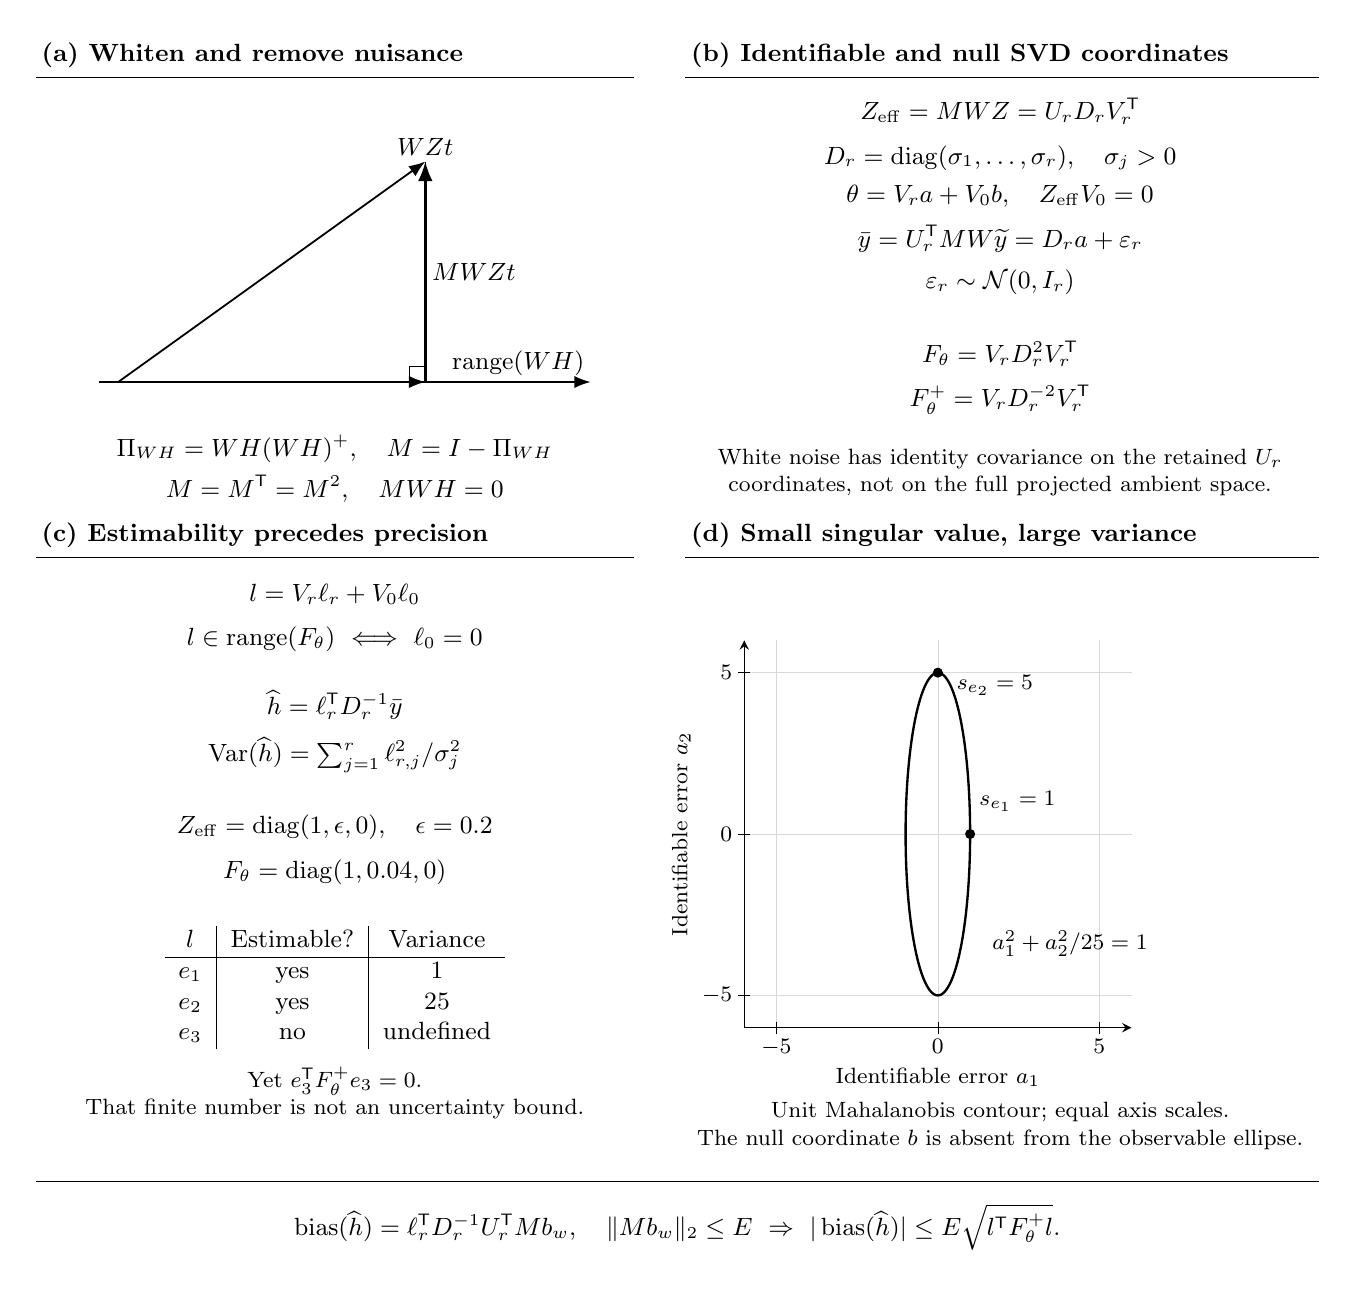
\begin{tikzpicture}[x=1cm,y=1cm]\path[use as bounding box] (0,0) rectangle (16.6,15.8);
\node[head] at (0.1,15.45){(a) Whiten and remove nuisance};\draw[wire] (0.1,15.17)--(7.699999999999999,15.17);
\node[head] at (8.35,15.45){(b) Identifiable and null SVD coordinates};\draw[wire] (8.35,15.17)--(16.4,15.17);
\draw[arr] (.9,11.3)--(7.15,11.3) node[above left] {$\range(WH)$};
\draw[arr] (1.15,11.3)--(5.05,14.1) node[above] {$WZt$};
\draw[dashed,wire] (5.05,11.3)--(5.05,14.1);
\draw[arr] (1.15,11.3)--(5.05,11.3);
\draw[arr,line width=.9pt] (5.05,11.3)--(5.05,14.1) node[midway,right] {$MWZt$};
\draw[wire] (4.85,11.3)--(4.85,11.5)--(5.05,11.5);
\node[eq] at (3.9,10.2){$\Pi_{WH}=WH(WH)^+,\quad M=I-\Pi_{WH}$\\[4pt]$M=M\trans=M^2,\quad MWH=0$};
\node[eq] at (12.35,14.45){$Z_{\mathrm{eff}}=MWZ=U_rD_rV_r\trans$\\[5pt]$D_r=\diag(\sigma_1,\ldots,\sigma_r),\quad\sigma_j>0$};
\node[eq] at (12.35,13.1){$\theta=V_ra+V_0b,\quad Z_{\mathrm{eff}}V_0=0$\\[5pt]
$\bar y=U_r\trans MW\widetilde y=D_ra+\varepsilon_r$\\[4pt]$\varepsilon_r\sim\mathcal N(0,I_r)$};
\node[eq] at (12.35,11.36){$F_\theta=V_rD_r^2V_r\trans$\\[5pt]$F_\theta^+=V_rD_r^{-2}V_r\trans$};
\node[tinytext,align=center] at (12.35,10.15){White noise has identity covariance on the retained $U_r$\\coordinates, not on the full projected ambient space.};
\node[head] at (0.1,9.35){(c) Estimability precedes precision};\draw[wire] (0.1,9.07)--(7.699999999999999,9.07);
\node[head] at (8.35,9.35){(d) Small singular value, large variance};\draw[wire] (8.35,9.07)--(16.4,9.07);
\node[eq] at (3.9,8.3){$l=V_r\ell_r+V_0\ell_0$\\[5pt]$l\in\range(F_\theta)\ \Longleftrightarrow\ \ell_0=0$};
\node[eq] at (3.9,6.86){$\widehat h=\ell_r\trans D_r^{-1}\bar y$\\[6pt]$\Var(\widehat h)=\sum_{j=1}^{r}\ell_{r,j}^2/\sigma_j^2$};
\node[eq] at (3.9,5.36){$Z_{\mathrm{eff}}=\diag(1,\epsilon,0),\quad\epsilon=0.2$\\[5pt]$F_\theta=\diag(1,0.04,0)$};
\node[eq] at (3.9,3.61){$\begin{array}{c|c|c}l&\text{Estimable?}&\text{Variance}\\\hline
e_1&\text{yes}&1\\e_2&\text{yes}&25\\e_3&\text{no}&\text{undefined}\end{array}$};
\node[tinytext,align=center] at (3.9,2.27){Yet $e_3\trans F_\theta^+e_3=0$.\\That finite number is not an uncertainty bound.};
\begin{axis}[mathaxis,axis equal image,at={(9.1cm,3.1cm)},anchor=south west,width=7.1cm,height=6.5cm,
 xmin=-6,xmax=6,ymin=-6,ymax=6,xtick={-5,0,5},ytick={-5,0,5},
 xlabel={Identifiable error $a_1$},ylabel={Identifiable error $a_2$},clip=false]
\addplot[domain=0:360,samples=121,line width=.85pt] ({cos(x)},{5*sin(x)});
\addplot[only marks,mark=*,mark size=1.6pt] coordinates {(1,0)(0,5)};
\node[anchor=west,tinytext] at (axis cs:.4,4.6){$s_{e_2}=5$};
\node[anchor=south west,tinytext] at (axis cs:1.1,.5){$s_{e_1}=1$};
\node[anchor=west,tinytext] at (axis cs:1.5,-3.4){$a_1^2+a_2^2/25=1$};\end{axis}
\node[tinytext,align=center] at (12.35,1.85){Unit Mahalanobis contour; equal axis scales.\\The null coordinate $b$ is absent from the observable ellipse.};
\draw[wire] (.1,1.15)--(16.4,1.15);
\node[eq] at (8.25,.57){$\operatorname{bias}(\widehat h)=\ell_r\trans D_r^{-1}U_r\trans Mb_w,\quad
\|Mb_w\|_2\leq E\ \Rightarrow\ |\operatorname{bias}(\widehat h)|\leq E\sqrt{l\trans F_\theta^+l}.$};
\end{tikzpicture}
\PlateCaption{\textbf{Figure 3.} Derivation of an estimable Gaussian target through whitening and orthogonal nuisance removal. Here $W\trans W=\Sigma^{-1}$ and $b_w=Wb_{\mathrm{mod}}$. The ellipse displays exact covariance in a normalized example, not physical-drive calibration. Small positive singular values amplify variance; a null target cannot be recovered by a pseudoinverse convention. The bias relation requires estimable $l$ and a justified whole-window discrepancy bound $E$.}

\newpage
\PlateTitle{4}{Shared dead time: the covariance eigenmode that actually diverges}
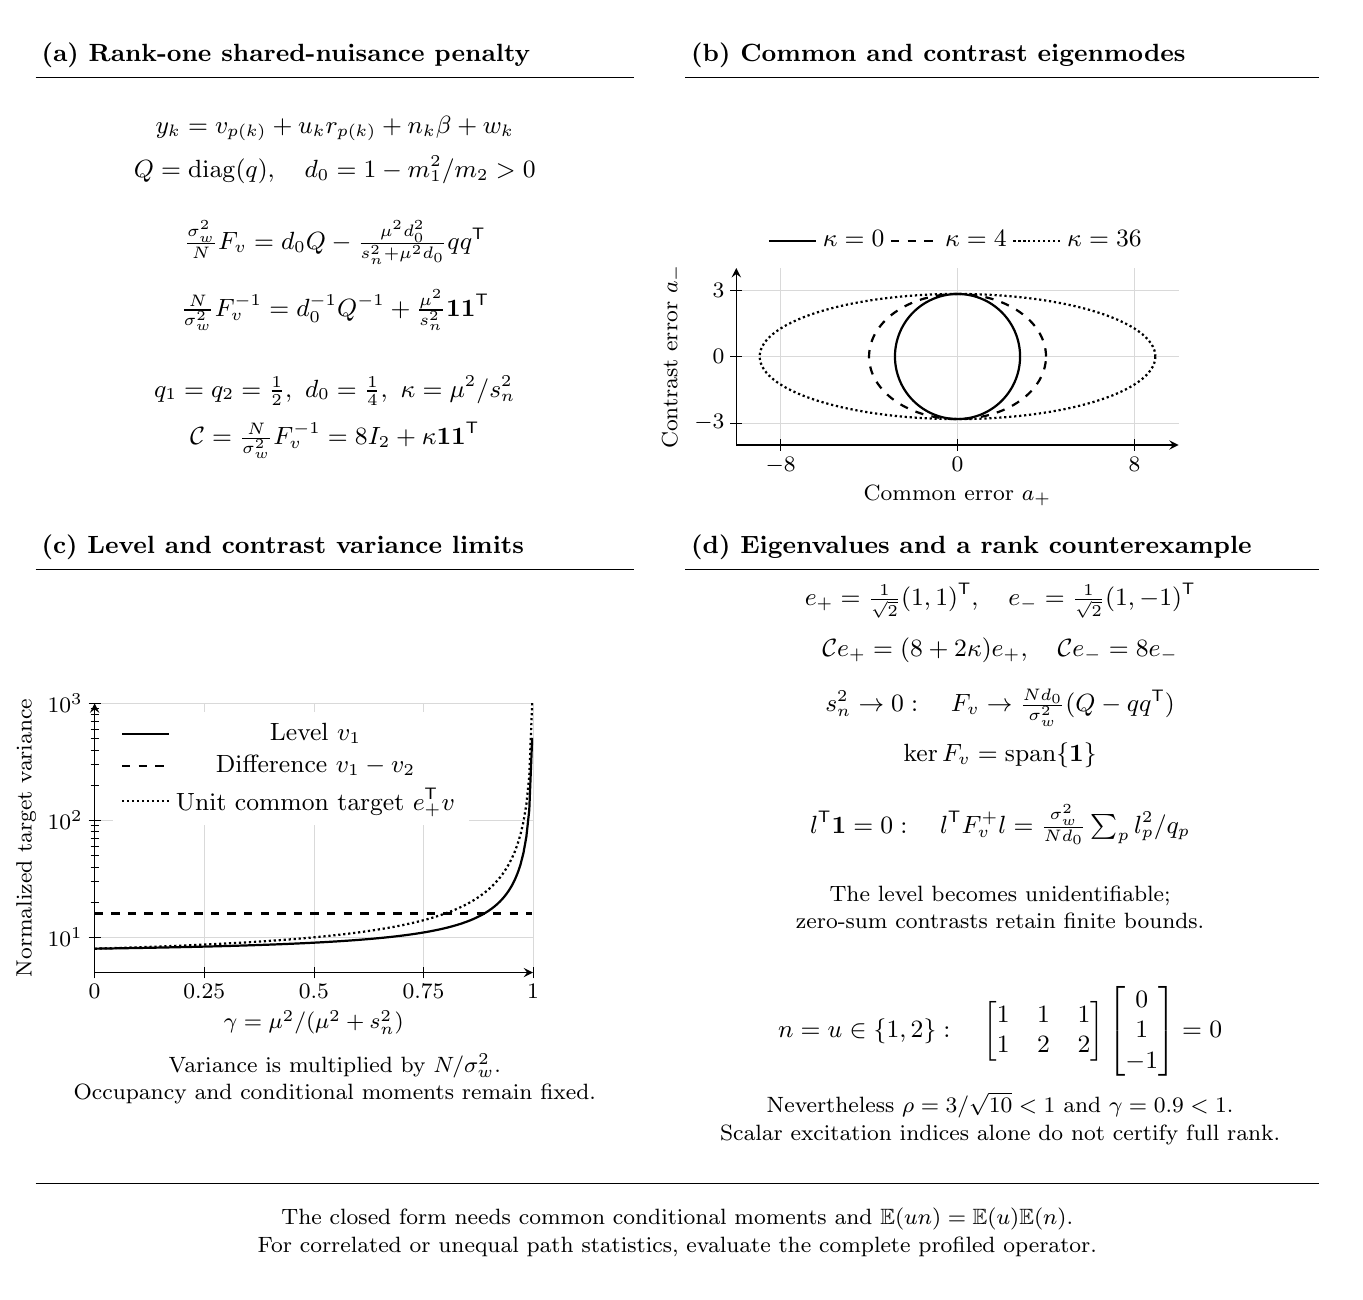
\begin{tikzpicture}[x=1cm,y=1cm]\path[use as bounding box] (0,0) rectangle (16.6,15.8);
\node[head] at (0.1,15.45){(a) Rank-one shared-nuisance penalty};\draw[wire] (0.1,15.17)--(7.699999999999999,15.17);
\node[head] at (8.35,15.45){(b) Common and contrast eigenmodes};\draw[wire] (8.35,15.17)--(16.4,15.17);
\node[eq] at (3.9,14.25){$y_k=v_{p(k)}+u_kr_{p(k)}+n_k\beta+w_k$\\[5pt]$Q=\diag(q),\quad d_0=1-m_1^2/m_2>0$};
\node[eq] at (3.9,12.65){$\frac{\sigma_w^2}{N}F_v=d_0Q-\frac{\mu^2d_0^2}{s_n^2+\mu^2d_0}qq\trans$\\[8pt]
$\frac{N}{\sigma_w^2}F_v^{-1}=d_0^{-1}Q^{-1}+\frac{\mu^2}{s_n^2}\one\one\trans$};
\node[eq] at (3.9,10.85){$q_1=q_2=\tfrac12,\ d_0=\tfrac14,\ \kappa=\mu^2/s_n^2$\\[5pt]
$\mathcal C=\frac{N}{\sigma_w^2}F_v^{-1}=8I_2+\kappa\one\one\trans$};
\begin{axis}[mathaxis,axis equal image,at={(9.0cm,10.5cm)},anchor=south west,width=7.2cm,height=4.2cm,
 xmin=-10,xmax=10,ymin=-4,ymax=4,xtick={-8,0,8},ytick={-3,0,3},
 xlabel={Common error $a_+$},ylabel={Contrast error $a_-$},legend style={at={(.5,1.03)},anchor=south,legend columns=3}]
\addplot[domain=0:360,samples=121,line width=.8pt] ({sqrt(8)*cos(x)},{sqrt(8)*sin(x)});\addlegendentry{$\kappa=0$}
\addplot[domain=0:360,samples=121,line width=.8pt,dashed] ({4*cos(x)},{sqrt(8)*sin(x)});\addlegendentry{$\kappa=4$}
\addplot[domain=0:360,samples=121,line width=.8pt,densely dotted] ({sqrt(80)*cos(x)},{sqrt(8)*sin(x)});\addlegendentry{$\kappa=36$}\end{axis}
\node[head] at (0.1,9.2){(c) Level and contrast variance limits};\draw[wire] (0.1,8.92)--(7.699999999999999,8.92);
\node[head] at (8.35,9.2){(d) Eigenvalues and a rank counterexample};\draw[wire] (8.35,8.92)--(16.4,8.92);
\begin{semilogyaxis}[mathaxis,at={(.85cm,3.8cm)},anchor=south west,width=7.15cm,height=5.0cm,
 xmin=0,xmax=1,ymin=5,ymax=1000,xtick={0,.25,.5,.75,1},ytick={10,100,1000},
 xlabel={$\gamma=\mu^2/(\mu^2+s_n^2)$},ylabel={Normalized target variance},legend style={at={(.04,.97)},anchor=north west}]
\addplot[domain=0:.998,samples=151,line width=.8pt]{8+x/(1-x)};\addlegendentry{Level $v_1$}
\addplot[domain=0:.998,samples=2,dashed,line width=.8pt]{16};\addlegendentry{Difference $v_1-v_2$}
\addplot[domain=0:.998,samples=151,densely dotted,line width=.8pt]{8+2*x/(1-x)};\addlegendentry{Unit common target $e_+\trans v$}\end{semilogyaxis}
\node[tinytext,align=center] at (3.9,2.45){Variance is multiplied by $N/\sigma_w^2$.\\Occupancy and conditional moments remain fixed.};
\node[eq] at (12.35,8.24){$e_+=\tfrac1{\sqrt2}(1,1)\trans,\quad e_-=\tfrac1{\sqrt2}(1,-1)\trans$\\[6pt]
$\mathcal C e_+=(8+2\kappa)e_+,\quad\mathcal C e_-=8e_-$};
\node[eq] at (12.35,6.9){$s_n^2\to0:\quad F_v\to\frac{Nd_0}{\sigma_w^2}(Q-qq\trans)$\\[5pt]$\ker F_v=\spanop\{\one\}$};
\node[eq] at (12.35,5.68){$l\trans\one=0:\quad l\trans F_v^+l=\frac{\sigma_w^2}{Nd_0}\sum_p l_p^2/q_p$};
\node[tinytext,align=center] at (12.35,4.63){The level becomes unidentifiable;\\zero-sum contrasts retain finite bounds.};
\node[eq] at (12.35,3.05){$n=u\in\{1,2\}:\quad\begin{bmatrix}1&1&1\\1&2&2\end{bmatrix}\begin{bmatrix}0\\1\\-1\end{bmatrix}=0$};
\node[tinytext,align=center] at (12.35,1.95){Nevertheless $\rho=3/\sqrt{10}<1$ and $\gamma=0.9<1$.\\Scalar excitation indices alone do not certify full rank.};
\draw[wire] (.1,1.12)--(16.4,1.12);
\node[tinytext,align=center] at (8.25,.5){The closed form needs common conditional moments and $\mathbb E(un)=\mathbb E(u)\mathbb E(n)$.\\For correlated or unequal path statistics, evaluate the complete profiled operator.};\end{tikzpicture}
\PlateCaption{\textbf{Figure 4.} Exact balanced two-path calculation with $d_0=1/4$. Unit Mahalanobis contours in (b) use the eigenbasis and units $\sigma_w/\sqrt N$. The rank-one term lengthens only the common coordinate. Panel (c) distinguishes an unnormalized difference from the unit common target. The counterexample violates moment factorization: resistance and dead-time columns coincide despite nondegenerate scalar moment indices. These are statistical design calculations, not measured drive operating curves.}

\newpage
\PlateTitle{5}{Thermal confounding as a kernel, and calibration uncertainty as a set}
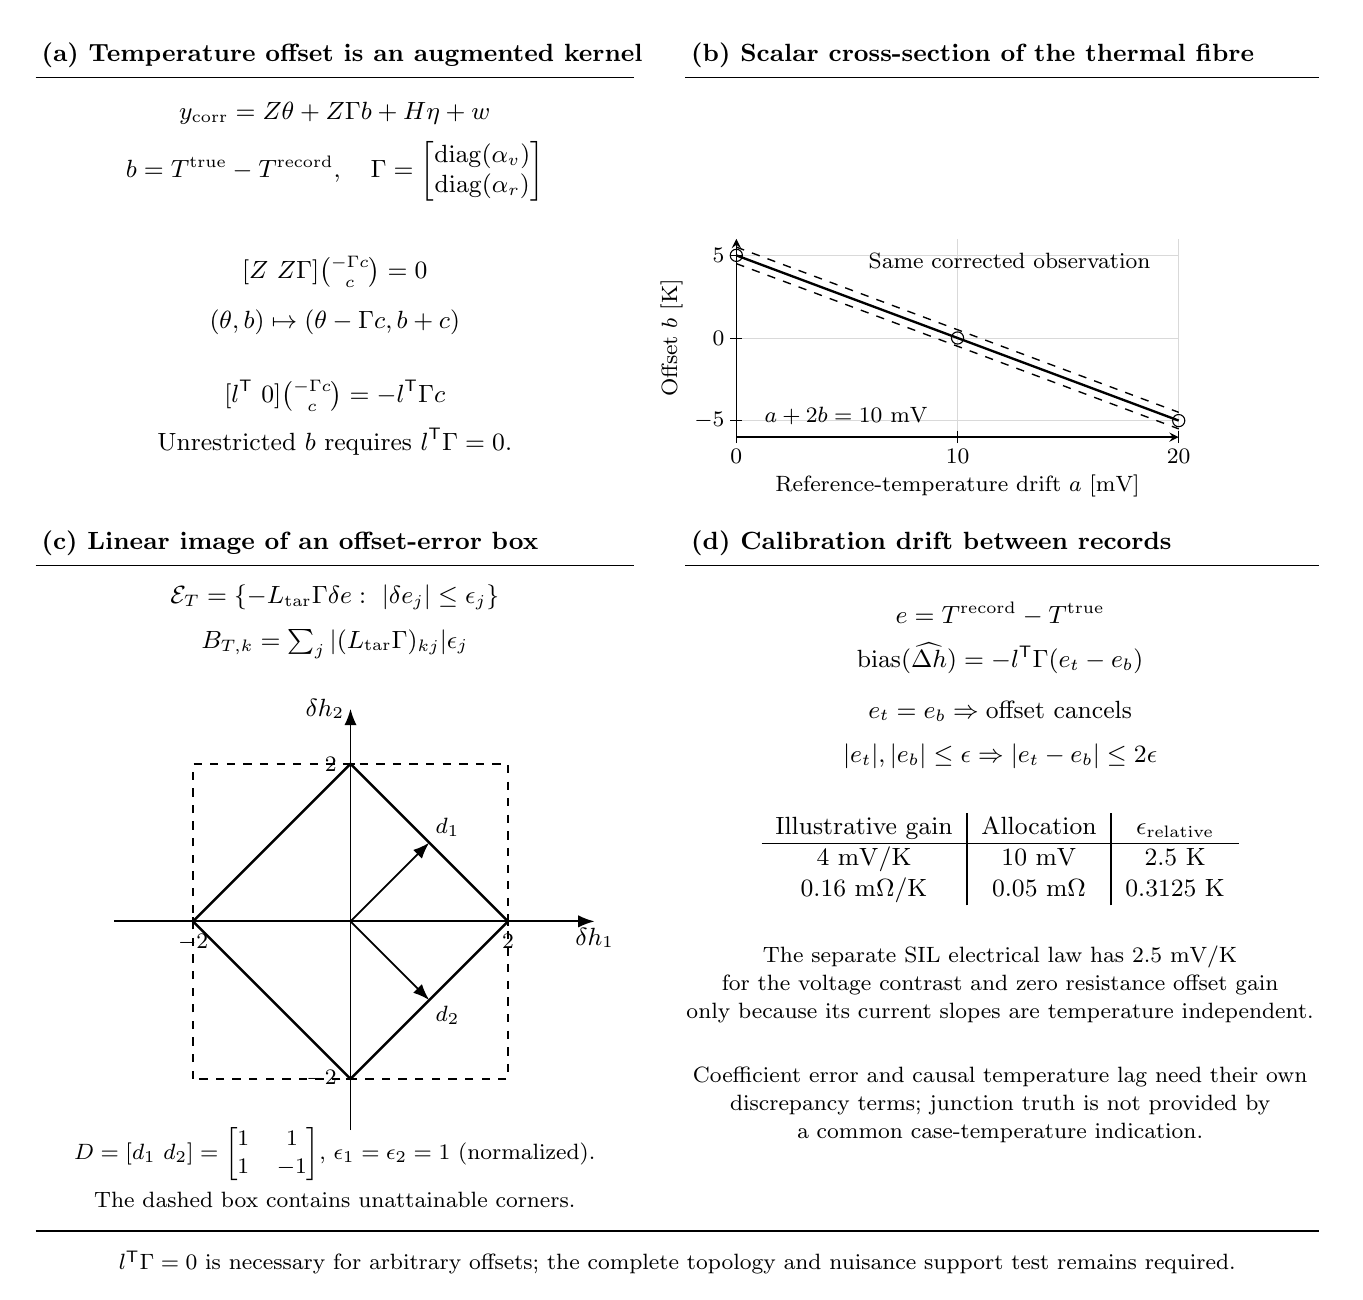
\begin{tikzpicture}[x=1cm,y=1cm]\path[use as bounding box] (0,0) rectangle (16.6,15.8);
\node[head] at (0.1,15.45){(a) Temperature offset is an augmented kernel};\draw[wire] (0.1,15.17)--(7.699999999999999,15.17);
\node[head] at (8.35,15.45){(b) Scalar cross-section of the thermal fibre};\draw[wire] (8.35,15.17)--(16.4,15.17);
\node[eq] at (3.9,14.22){$y_{\mathrm{corr}}=Z\theta+Z\Gamma b+H\eta+w$\\[5pt]
$b=T^{\mathrm{true}}-T^{\mathrm{record}},\quad\Gamma=\begin{bmatrix}\diag(\alpha_v)\\\diag(\alpha_r)\end{bmatrix}$};
\node[eq] at (3.9,12.4){$[Z\ Z\Gamma]\binom{-\Gamma c}{c}=0$\\[7pt]$(\theta,b)\mapsto(\theta-\Gamma c,b+c)$};
\node[eq] at (3.9,10.85){$[l\trans\ 0]\binom{-\Gamma c}{c}=-l\trans\Gamma c$\\[5pt]Unrestricted $b$ requires $l\trans\Gamma=0$.};
\begin{axis}[mathaxis,at={(9.0cm,10.6cm)},anchor=south west,width=7.2cm,height=4.1cm,
 xmin=0,xmax=20,ymin=-6,ymax=6,xtick={0,10,20},ytick={-5,0,5},
 xlabel={Reference-temperature drift $a$ [mV]},ylabel={Offset $b$ [K]},clip=false]
\addplot[domain=0:20,samples=2,line width=.85pt]{(10-x)/2};
\addplot[domain=0:20,samples=2,dashed,line width=.5pt]{(11-x)/2};
\addplot[domain=0:20,samples=2,dashed,line width=.5pt]{(9-x)/2};
\addplot[only marks,mark=o,mark size=2.2pt] coordinates {(0,5)(10,0)(20,-5)};
\node[tinytext,anchor=west] at (axis cs:1,-4.7){$a+2b=10$ mV};
\node[tinytext,anchor=east] at (axis cs:19,4.7){Same corrected observation};\end{axis}
\node[head] at (0.1,9.25){(c) Linear image of an offset-error box};\draw[wire] (0.1,8.97)--(7.699999999999999,8.97);
\node[head] at (8.35,9.25){(d) Calibration drift between records};\draw[wire] (8.35,8.97)--(16.4,8.97);
\node[eq] at (3.9,8.25){$\mathcal E_T=\{-L_{\mathrm{tar}}\Gamma\delta e:\ |\delta e_j|\leq\epsilon_j\}$\\[5pt]
$B_{T,k}=\sum_j |(L_{\mathrm{tar}}\Gamma)_{kj}|\epsilon_j$};
\draw[arr] (1.1,4.45)--(7.2,4.45) node[below] {$\delta h_1$};
\draw[arr] (4.1,1.8)--(4.1,7.15) node[left] {$\delta h_2$};
\draw[dashed,wire] (2.1,2.45) rectangle (6.1,6.45);
\draw[line width=.9pt] (2.1,4.45)--(4.1,6.45)--(6.1,4.45)--(4.1,2.45)--cycle;
\draw[arr] (4.1,4.45)--(5.1,5.45) node[above right,tinytext] {$d_1$};
\draw[arr] (4.1,4.45)--(5.1,3.45) node[below right,tinytext] {$d_2$};
\foreach \xx/\lab in {2.1/-2,6.1/2}{\draw[wire] (\xx,4.39)--(\xx,4.51);\node[tinytext,below] at (\xx,4.37){$\lab$};}
\foreach \yy/\lab in {2.45/-2,6.45/2}{\draw[wire] (4.04,\yy)--(4.16,\yy);\node[tinytext,left] at (4.0,\yy){$\lab$};}
\node[tinytext,align=center] at (3.9,1.5){$D=[d_1\ d_2]=\begin{bmatrix}1&1\\1&-1\end{bmatrix}$, $\epsilon_1=\epsilon_2=1$ (normalized).};
\node[tinytext] at (3.9,.92){The dashed box contains unattainable corners.};
\node[eq] at (12.35,8.05){$e=T^{\mathrm{record}}-T^{\mathrm{true}}$\\[5pt]$\operatorname{bias}(\widehat{\Delta h})=-l\trans\Gamma(e_t-e_b)$};
\node[eq] at (12.35,6.82){$e_t=e_b\Rightarrow\text{offset cancels}$\\[5pt]$|e_t|,|e_b|\leq\epsilon\Rightarrow|e_t-e_b|\leq2\epsilon$};
\node[eq] at (12.35,5.24){$\begin{array}{c|c|c}\text{Illustrative gain}&\text{Allocation}&\epsilon_{\mathrm{relative}}\\\hline
4\ \mathrm{mV/K}&10\ \mathrm{mV}&2.5\ \mathrm K\\0.16\ \mathrm{m}\Omega/\mathrm K&0.05\ \mathrm{m}\Omega&0.3125\ \mathrm K\end{array}$};
\node[tinytext,align=center] at (12.35,3.65){The separate SIL electrical law has 2.5 mV/K\\for the voltage contrast and zero resistance offset gain\\only because its current slopes are temperature independent.};
\node[tinytext,align=center] at (12.35,2.12){Coefficient error and causal temperature lag need their own\\discrepancy terms; junction truth is not provided by\\a common case-temperature indication.};
\draw[wire] (.1,.52)--(16.4,.52);
\node[tinytext] at (8.25,.12){$l\trans\Gamma=0$ is necessary for arbitrary offsets; the complete topology and nuisance support test remains required.};\end{tikzpicture}
\PlateCaption{\textbf{Figure 5.} Unbounded offsets create an exact equivalence; bounded relative offsets create a deterministic target-error set. In (b), $\alpha=2$ mV/K and the 10 mV observation are analytic settings; dashed lines mark a hypothetical $\pm1$ mV observation band, not measured noise. The diamond is a normalized linear image of an offset box. Numerical allocations belong to the illustrative law and are separated from the SIL surrogate. They are conditional budgets, not demonstrated sensor accuracies.}

\newpage
\PlateTitle{6}{Baseline covariance, calibration rank and power of the actual task}
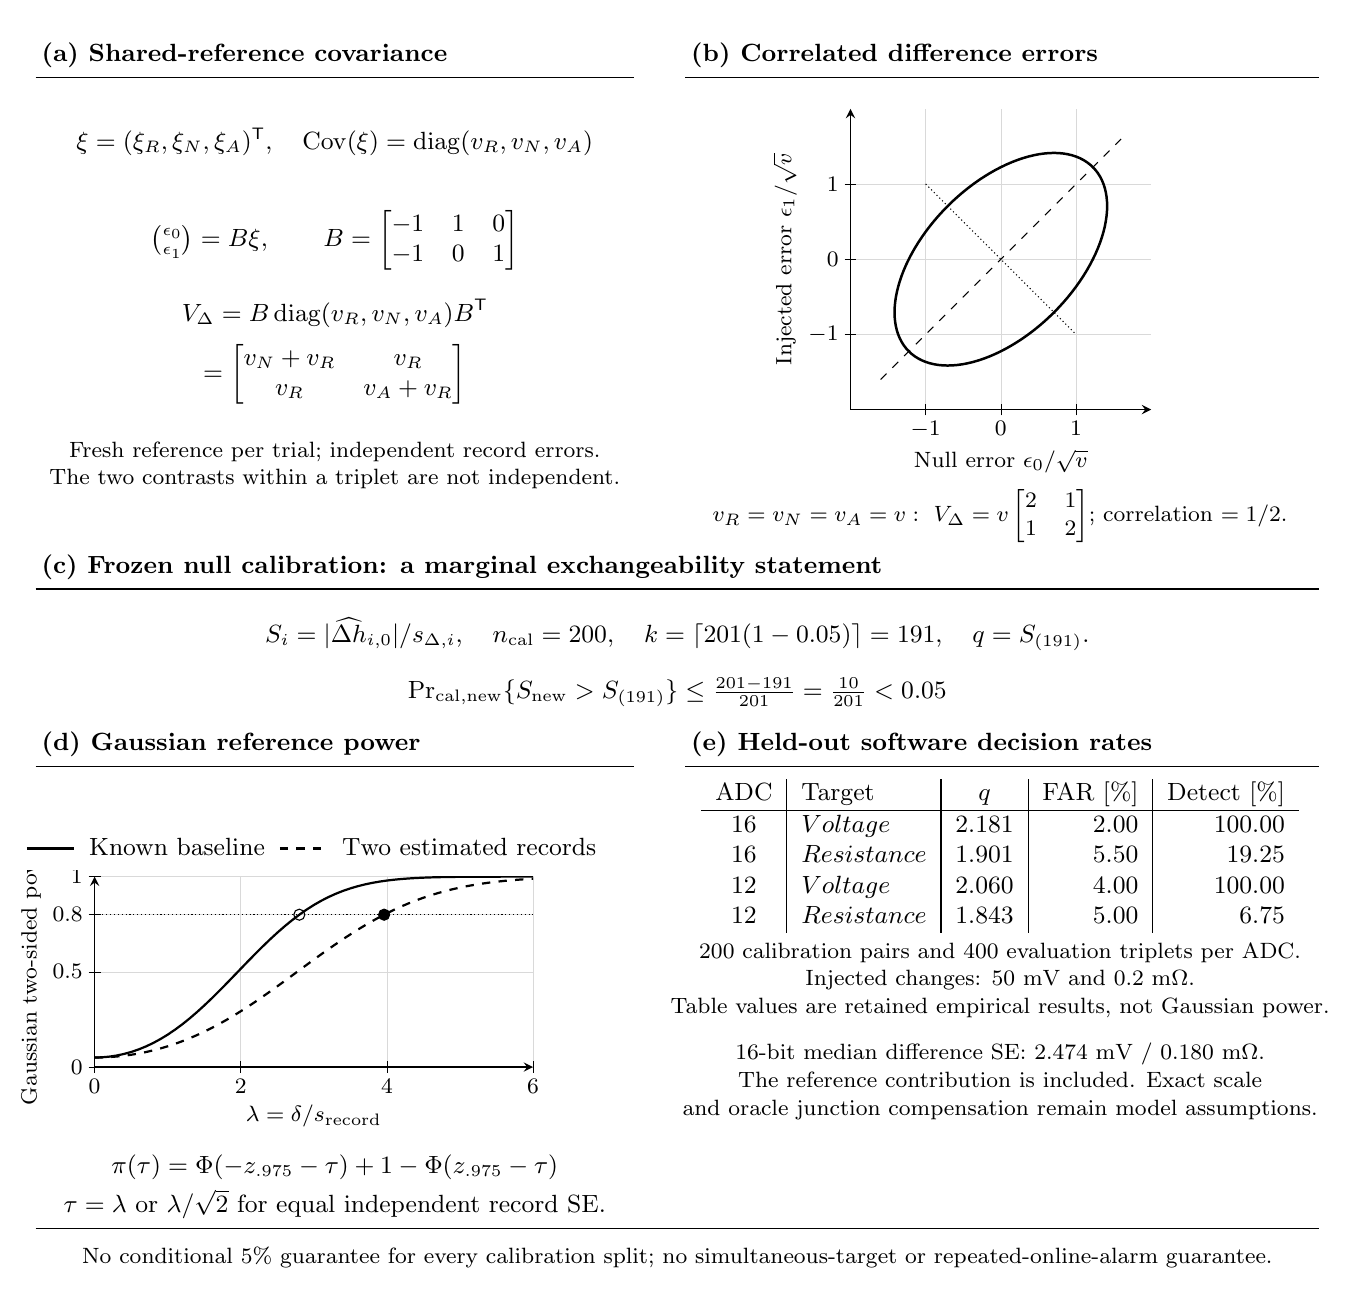
\begin{tikzpicture}[x=1cm,y=1cm]\path[use as bounding box] (0,0) rectangle (16.6,15.8);
\node[head] at (0.1,15.45){(a) Shared-reference covariance};\draw[wire] (0.1,15.17)--(7.699999999999999,15.17);
\node[head] at (8.35,15.45){(b) Correlated difference errors};\draw[wire] (8.35,15.17)--(16.4,15.17);
\node[eq] at (3.9,14.35){$\xi=(\xi_R,\xi_N,\xi_A)\trans,\quad\Cov(\xi)=\diag(v_R,v_N,v_A)$};
\node[eq] at (3.9,13.1){$\binom{\epsilon_0}{\epsilon_1}=B\xi,\qquad B=\begin{bmatrix}-1&1&0\\-1&0&1\end{bmatrix}$};
\node[eq] at (3.9,11.68){$V_\Delta=B\diag(v_R,v_N,v_A)B\trans$\\[5pt]$=\begin{bmatrix}v_N+v_R&v_R\\v_R&v_A+v_R\end{bmatrix}$};
\node[tinytext,align=center] at (3.9,10.24){Fresh reference per trial; independent record errors.\\The two contrasts within a triplet are not independent.};
\begin{axis}[mathaxis,axis equal image,at={(10.45cm,10.95cm)},anchor=south west,width=7.2cm,height=5.4cm,
 xmin=-2,xmax=2,ymin=-2,ymax=2,xtick={-1,0,1},ytick={-1,0,1},
 xlabel={Null error $\epsilon_0/\sqrt v$},ylabel={Injected error $\epsilon_1/\sqrt v$},clip=false]
\addplot[domain=0:360,samples=121,line width=.9pt]
 ({(sqrt(3)*cos(x)+sin(x))/sqrt(2)},{(sqrt(3)*cos(x)-sin(x))/sqrt(2)});
\addplot[domain=-1.6:1.6,samples=2,dashed]{x};
\addplot[domain=-1:1,samples=2,densely dotted]{-x};\end{axis}
\node[tinytext,align=center] at (12.35,9.6){$v_R=v_N=v_A=v:\ V_\Delta=v\begin{bmatrix}2&1\\1&2\end{bmatrix}$; correlation $=1/2$.};
\node[head] at (0.1,8.95){(c) Frozen null calibration: a marginal exchangeability statement};\draw[wire] (0.1,8.67)--(16.400000000000002,8.67);
\node[eq] at (8.25,8.1){$S_i=|\widehat{\Delta h}_{i,0}|/s_{\Delta,i},\quad n_{\mathrm{cal}}=200,\quad
k=\lceil201(1-0.05)\rceil=191,\quad q=S_{(191)}.$};
\node[eq] at (8.25,7.36){$\Pr_{\mathrm{cal,new}}\{S_{\mathrm{new}}>S_{(191)}\}\leq\frac{201-191}{201}=\frac{10}{201}<0.05$};
\node[head] at (0.1,6.7){(d) Gaussian reference power};\draw[wire] (0.1,6.42)--(7.699999999999999,6.42);
\node[head] at (8.35,6.7){(e) Held-out software decision rates};\draw[wire] (8.35,6.42)--(16.4,6.42);
\begin{axis}[mathaxis,at={(.85cm,2.6cm)},anchor=south west,width=7.15cm,height=4.0cm,
 xmin=0,xmax=6,ymin=0,ymax=1,xtick={0,2,4,6},ytick={0,.5,.8,1},
 xlabel={$\lambda=\delta/s_{\mathrm{record}}$},ylabel={Gaussian two-sided power},
 legend style={at={(.5,1.03)},anchor=south,legend columns=2,/tikz/column sep=3pt}]
\addplot[line width=.8pt,solid] coordinates {(0.000000,0.05000000) (0.100000,0.05114630) (0.200000,0.05459469) (0.300000,0.06037259) (0.400000,0.06852255) (0.500000,0.07909753) (0.600000,0.09215481) (0.700000,0.10774863) (0.800000,0.12592212) (0.900000,0.14669894) (1.000000,0.17007505) (1.100000,0.19601127) (1.200000,0.22442700) (1.300000,0.25519560) (1.400000,0.28814177) (1.500000,0.32304116) (1.600000,0.35962249) (1.700000,0.39757190) (1.800000,0.43653969) (1.900000,0.47614886) (2.000000,0.51600527) (2.100000,0.55570877) (2.200000,0.59486475) (2.300000,0.63309552) (2.400000,0.67005099) (2.500000,0.70541800) (2.600000,0.73892797) (2.700000,0.77036251) (2.800000,0.79955687) (2.900000,0.82640104) (3.000000,0.85083877) (3.100000,0.87286456) (3.200000,0.89251909) (3.300000,0.90988325) (3.400000,0.92507144) (3.500000,0.93822424) (3.600000,0.94950117) (3.700000,0.95907366) (3.800000,0.96711853) (3.900000,0.97381235) (4.000000,0.97932663) (4.100000,0.98382407) (4.200000,0.98745571) (4.300000,0.99035906) (4.400000,0.99265710) (4.500000,0.99445795) (4.600000,0.99585514) (4.700000,0.99692838) (4.800000,0.99774458) (4.900000,0.99835913) (5.000000,0.99881725) (5.100000,0.99915536) (5.200000,0.99940243) (5.300000,0.99958116) (5.400000,0.99970918) (5.500000,0.99979996) (5.600000,0.99986370) (5.700000,0.99990800) (5.800000,0.99993849) (5.900000,0.99995927) (6.000000,0.99997328)};\addlegendentry{Known baseline}
\addplot[line width=.8pt,dashed] coordinates {(0.000000,0.05000000) (0.100000,0.05057295) (0.200000,0.05229420) (0.300000,0.05517078) (0.400000,0.05921403) (0.500000,0.06443897) (0.600000,0.07086349) (0.700000,0.07850736) (0.800000,0.08739098) (0.900000,0.09753416) (1.000000,0.10895462) (1.100000,0.12166654) (1.200000,0.13567910) (1.300000,0.15099497) (1.400000,0.16760895) (1.500000,0.18550670) (1.600000,0.20466363) (1.700000,0.22504400) (1.800000,0.24660025) (1.900000,0.26927261) (2.000000,0.29298894) (2.100000,0.31766497) (2.200000,0.34320476) (2.300000,0.36950147) (2.400000,0.39643844) (2.500000,0.42389054) (2.600000,0.45172572) (2.700000,0.47980674) (2.800000,0.50799315) (2.900000,0.53614322) (3.000000,0.56411603) (3.100000,0.59177351) (3.200000,0.61898244) (3.300000,0.64561631) (3.400000,0.67155705) (3.500000,0.69669656) (3.600000,0.72093800) (3.700000,0.74419681) (3.800000,0.76640150) (3.900000,0.78749412) (4.000000,0.80743042) (4.100000,0.82617984) (4.200000,0.84372510) (4.300000,0.86006167) (4.400000,0.87519698) (4.500000,0.88914945) (4.600000,0.90194738) (4.700000,0.91362779) (4.800000,0.92423511) (4.900000,0.93381989) (5.000000,0.94243754) (5.100000,0.95014701) (5.200000,0.95700963) (5.300000,0.96308795) (5.400000,0.96844478) (5.500000,0.97314222) (5.600000,0.97724091) (5.700000,0.98079932) (5.800000,0.98387327) (5.900000,0.98651549) (6.000000,0.98877529)};\addlegendentry{Two estimated records}
\addplot[densely dotted,domain=0:6,samples=2,forget plot]{.8};
\addplot[only marks,mark=o,mark size=2pt,forget plot] coordinates {(2.801582,.8)};
\addplot[only marks,mark=*,mark size=2pt,forget plot] coordinates {(3.962034,.8)};
\end{axis}
\node[eq] at (3.9,1.08){$\pi(\tau)=\Phi(-z_{.975}-\tau)+1-\Phi(z_{.975}-\tau)$\\[3pt]
$\tau=\lambda\text{ or }\lambda/\sqrt2$ for equal independent record SE.};
\node[eq] at (12.35,5.28){$\begin{array}{c|l|c|r|r}\text{ADC}&\text{Target}&q&\text{FAR [\%]}&\text{Detect [\%]}\\\hline
16&Voltage&2.181&2.00&100.00\\
16&Resistance&1.901&5.50&19.25\\
12&Voltage&2.060&4.00&100.00\\
12&Resistance&1.843&5.00&6.75\\\end{array}$};
\node[tinytext,align=center] at (12.35,3.7){200 calibration pairs and 400 evaluation triplets per ADC.\\Injected changes: 50 mV and 0.2 m$\Omega$.\\Table values are retained empirical results, not Gaussian power.};
\node[tinytext,align=center] at (12.35,2.42){16-bit median difference SE: 2.474 mV / 0.180 m$\Omega$.\\The reference contribution is included. Exact scale\\and oracle junction compensation remain model assumptions.};
\draw[wire] (.1,.55)--(16.4,.55);
\node[tinytext] at (8.25,.18){No conditional 5\% guarantee for every calibration split; no simultaneous-target or repeated-online-alarm guarantee.};\end{tikzpicture}
\PlateCaption{\textbf{Figure 6.} Independent record errors induce within-triplet correlation; exchangeable null scores justify finite-rank calibration per target and ADC. The ellipse is a unit Mahalanobis contour. In (d), 80\% Gaussian power requires $\lambda\simeq2.80$ with a known baseline and $\lambda\simeq3.96$ with two equally precise independent estimates. Panel (e) reports empirical software results from quantized feedback, separately from Gaussian power. Neither calculation establishes physical calibration or online alarm validity.}

\newpage
\PlateTitle{7}{Excitation is an angle: visualize information before collecting more samples}
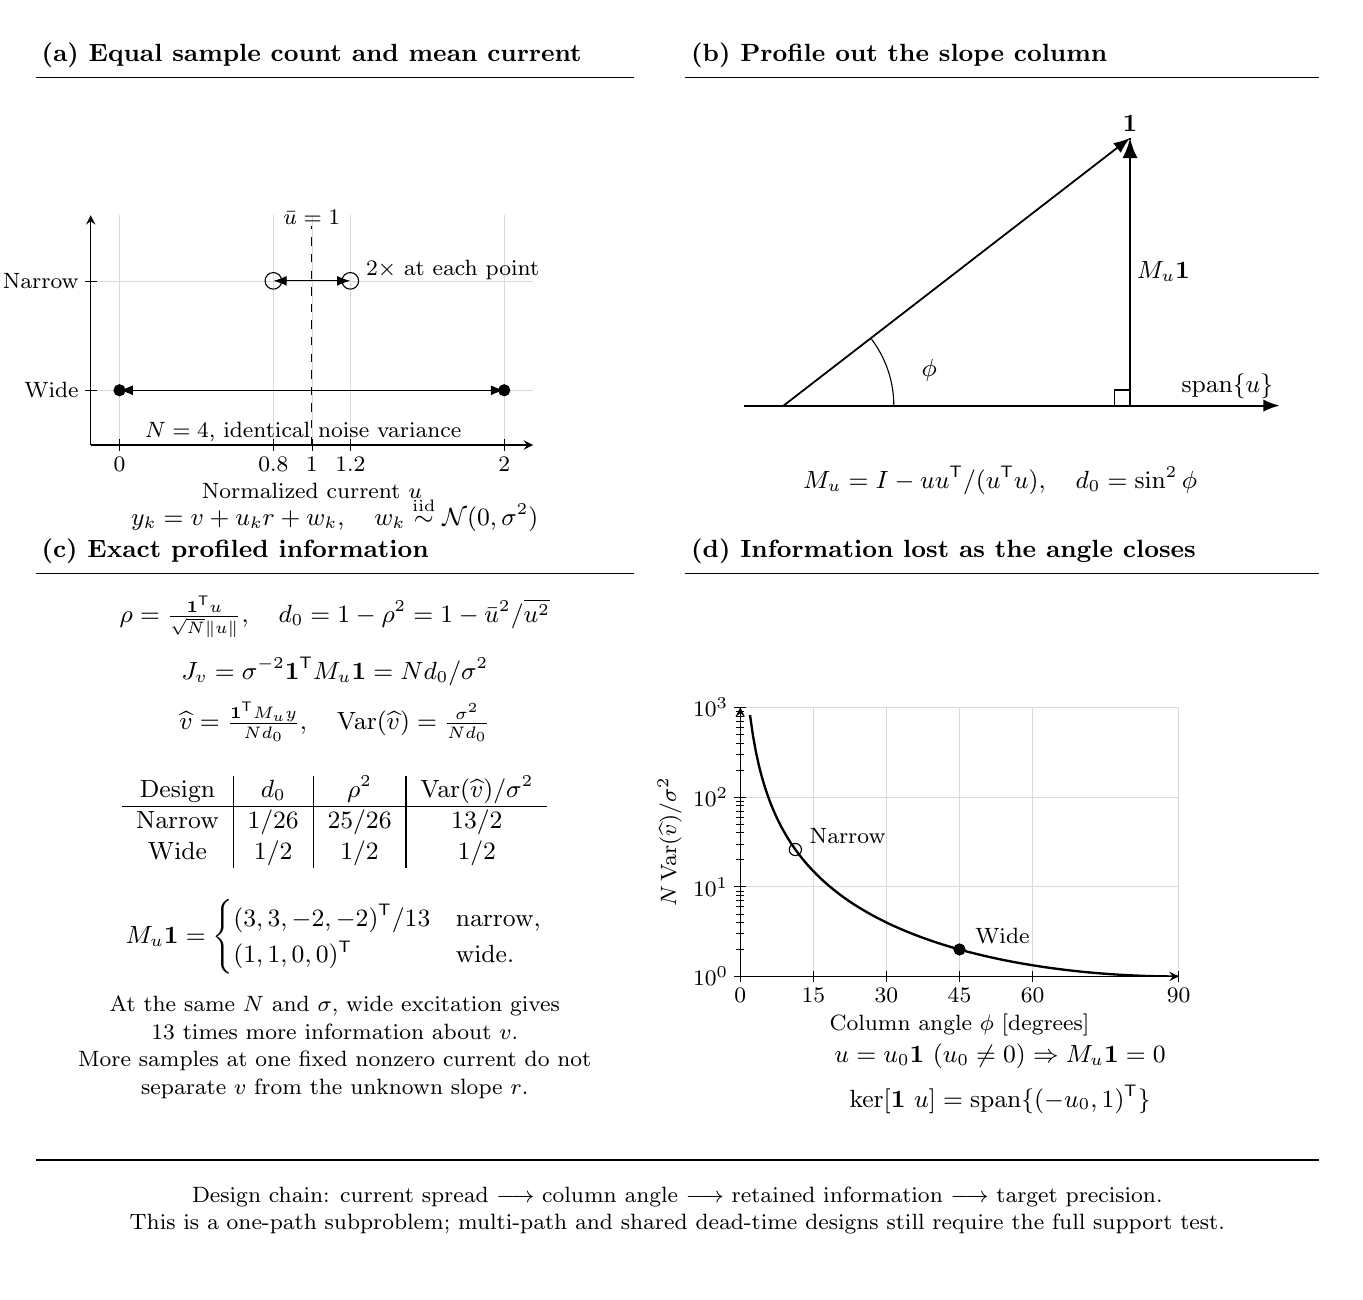
\begin{tikzpicture}[x=1cm,y=1cm]\path[use as bounding box] (0,0) rectangle (16.6,15.8);
\node[head] at (0.1,15.45){(a) Equal sample count and mean current};\draw[wire] (0.1,15.17)--(7.699999999999999,15.17);
\node[head] at (8.35,15.45){(b) Profile out the slope column};\draw[wire] (8.35,15.17)--(16.4,15.17);
\begin{axis}[mathaxis,at={(.8cm,10.5cm)},anchor=south west,width=7.2cm,height=4.5cm,
 xmin=-.15,xmax=2.15,ymin=.1,ymax=1.15,xtick={0,.8,1,1.2,2},ytick={.35,.85},yticklabels={Wide,Narrow},
 xlabel={Normalized current $u$},ylabel={Design},clip=false]
\addplot[only marks,mark=o,mark size=3pt] coordinates {(.8,.85)(1.2,.85)};
\addplot[only marks,mark=*,mark size=2pt] coordinates {(0,.35)(2,.35)};
\draw[<->] (axis cs:.8,.85)--(axis cs:1.2,.85);
\draw[<->] (axis cs:0,.35)--(axis cs:2,.35);
\draw[dashed] (axis cs:1,.1)--(axis cs:1,1.1);
\node[tinytext,anchor=south] at (axis cs:1,1.08){$\bar u=1$};
\node[tinytext,anchor=west] at (axis cs:1.25,.9){$2\times$ at each point};
\node[tinytext,anchor=west] at (axis cs:.1,.16){$N=4$, identical noise variance};\end{axis}
\node[eq] at (3.9,9.62){$y_k=v+u_kr+w_k,\quad w_k\overset{\mathrm{iid}}\sim\mathcal N(0,\sigma^2)$};
\draw[arr] (9.1,11.0)--(15.9,11.0) node[above left] {$\spanop\{u\}$};
\draw[arr] (9.6,11.0)--(14.0,14.4) node[above] {$\one$};
\draw[dashed,wire] (14,11)--(14,14.4);
\draw[arr,line width=.95pt] (14,11)--(14,14.4) node[right,midway] {$M_u\one$};
\draw[wire] (13.8,11)--(13.8,11.2)--(14,11.2);
\draw (11,11) arc[start angle=0,end angle=37.7,radius=1.4];
\node at (11.45,11.45){$\phi$};
\node[eq] at (12.35,10.05){$M_u=I-uu\trans/(u\trans u),\quad d_0=\sin^2\phi$};
\node[head] at (0.1,9.15){(c) Exact profiled information};\draw[wire] (0.1,8.870000000000001)--(7.699999999999999,8.870000000000001);
\node[head] at (8.35,9.15){(d) Information lost as the angle closes};\draw[wire] (8.35,8.870000000000001)--(16.4,8.870000000000001);
\node[eq] at (3.9,8.32){$\rho=\frac{\one\trans u}{\sqrt{N}\|u\|},\quad d_0=1-\rho^2=1-\bar u^2/\overline{u^2}$};
\node[eq] at (3.9,7.27){$J_v=\sigma^{-2}\one\trans M_u\one=Nd_0/\sigma^2$\\[5pt]
$\widehat v=\frac{\one\trans M_uy}{Nd_0},\quad\Var(\widehat v)=\frac{\sigma^2}{Nd_0}$};
\node[eq] at (3.9,5.71){$\begin{array}{c|c|c|c}\text{Design}&d_0&\rho^2&\Var(\widehat v)/\sigma^2\\\hline
\text{Narrow}&1/26&25/26&13/2\\\text{Wide}&1/2&1/2&1/2\end{array}$};
\node[eq] at (3.9,4.25){$M_u\one=\begin{cases}(3,3,-2,-2)\trans/13&\text{narrow},\\(1,1,0,0)\trans&\text{wide}.\end{cases}$};
\node[tinytext,align=center] at (3.9,2.85){At the same $N$ and $\sigma$, wide excitation gives\\13 times more information about $v$.\\More samples at one fixed nonzero current do not\\separate $v$ from the unknown slope $r$.};
\begin{semilogyaxis}[mathaxis,at={(9.05cm,3.75cm)},anchor=south west,width=7.15cm,height=5.0cm,
 xmin=0,xmax=90,ymin=1,ymax=1000,xtick={0,15,30,45,60,90},ytick={1,10,100,1000},
 xlabel={Column angle $\phi$ [degrees]},ylabel={$N\Var(\widehat v)/\sigma^2$}]
\addplot[domain=2:90,samples=150,line width=.85pt]{1/(sin(x)^2)};
\addplot[only marks,mark=o,mark size=2.2pt] coordinates {(11.309932,26)};
\addplot[only marks,mark=*,mark size=2pt] coordinates {(45,2)};
\node[tinytext,anchor=south west] at (axis cs:13,26){Narrow};
\node[tinytext,anchor=south west] at (axis cs:47,2){Wide};\end{semilogyaxis}
\node[eq] at (12.35,2.45){$u=u_0\one\ (u_0\neq0)\Rightarrow M_u\one=0$\\[5pt]
$\ker[\one\ u]=\spanop\{(-u_0,1)\trans\}$};
\draw[wire] (.1,1.42)--(16.4,1.42);
\node[tinytext,align=center] at (8.25,.78){Design chain: current spread $\longrightarrow$ column angle $\longrightarrow$ retained information $\longrightarrow$ target precision.\\This is a one-path subproblem; multi-path and shared dead-time designs still require the full support test.};
\end{tikzpicture}
\PlateCaption{\textbf{Figure 7.} Analytic two-regressor experiment, with four samples and an unknown resistance slope. Duplicate marks denote repeated inputs, not hidden data. The observation-space sketch illustrates an orthogonal decomposition; numerical angles and variance factors are calculated exactly from the displayed designs. The zero-current-only design needs separate handling because the slope column vanishes. No hardware trajectory or operating recommendation is inferred from this normalized example.}

\newpage
\PlateTitle{8}{See the quotient: a bounded target inside an unbounded likelihood tube}
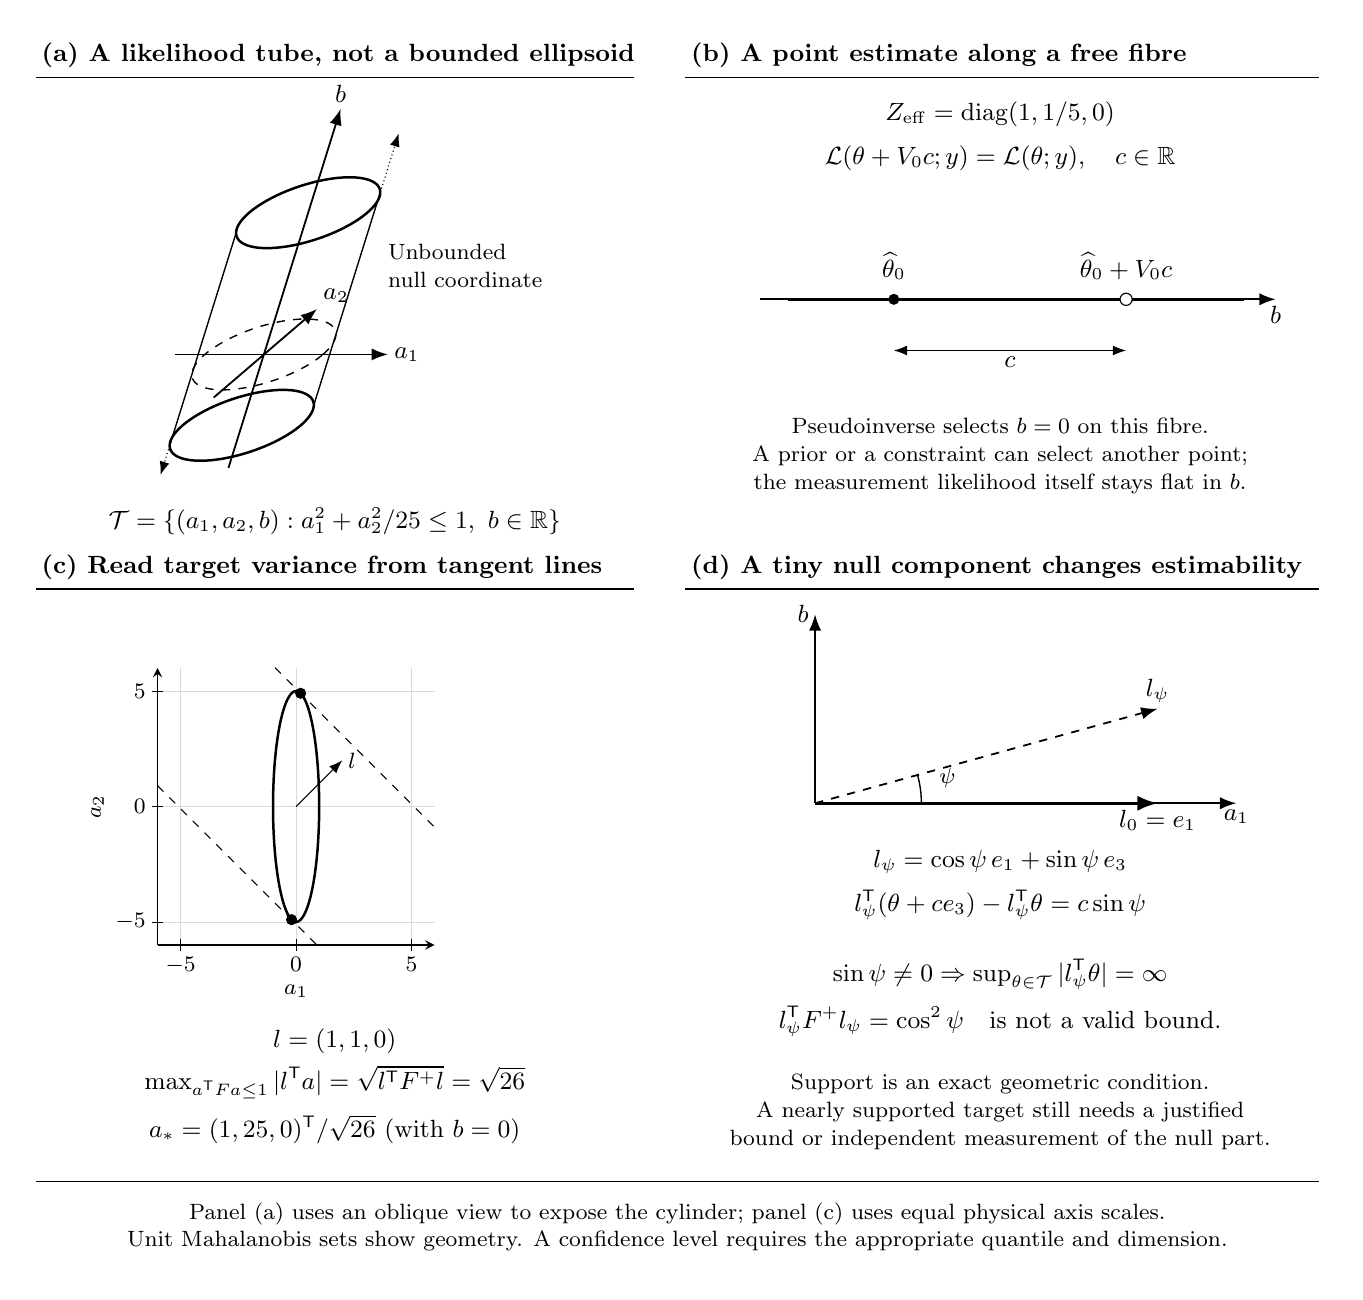
\begin{tikzpicture}[x=1cm,y=1cm]\path[use as bounding box] (0,0) rectangle (16.6,15.8);
\node[head] at (0.1,15.45){(a) A likelihood tube, not a bounded ellipsoid};\draw[wire] (0.1,15.17)--(7.699999999999999,15.17);
\node[head] at (8.35,15.45){(b) A point estimate along a free fibre};\draw[wire] (8.35,15.17)--(16.4,15.17);
\begin{scope}[shift={(3.0,11.65)},scale=.75]
\draw[arr] (-1.5,0)--(2.1,0) node[right] {$a_1$};
\draw[arr] (-.85,-.73)--(.9,.77) node[above right] {$a_2$};
\draw[arr] (-.6,-1.92)--(1.3,4.16) node[above] {$b$};
\draw[dashed,wire] plot[domain=0:360,samples=100] ({cos(\x)+.7*sin(\x)},{.6*sin(\x)});
\draw[line width=.9pt] plot[domain=0:360,samples=100] ({.75+cos(\x)+.7*sin(\x)},{2.4+.6*sin(\x)});
\draw[line width=.9pt] plot[domain=0:360,samples=100] ({-.375+cos(\x)+.7*sin(\x)},{-1.2+.6*sin(\x)});
\draw[wire] (-1.596,-1.544)--(-.471,2.056);
\draw[wire] (.846,-.856)--(1.971,2.744);
\draw[densely dotted,->] (1.971,2.744)--(2.284,3.744);
\draw[densely dotted,->] (-1.596,-1.544)--(-1.75,-2.04);
\node[tinytext,align=left,anchor=west] at (2.0,1.5){Unbounded\\null coordinate};
\end{scope}
\node[eq] at (3.9,9.53){$\mathcal T=\{(a_1,a_2,b):a_1^2+a_2^2/25\leq1,\ b\in\R\}$};
\draw[arr] (9.3,12.35)--(15.85,12.35) node[below] {$b$};
\draw[line width=.95pt] (9.65,12.35)--(15.45,12.35);
\fill (11.0,12.35) circle(2pt);\draw[fill=white] (13.95,12.35) circle(2.2pt);
\node[above] at (11,12.52){$\widehat\theta_0$};\node[above] at (13.95,12.52){$\widehat\theta_0+V_0c$};
\draw[<->] (11,11.7)--(13.95,11.7) node[midway,below] {$c$};
\node[eq] at (12.35,14.42){$Z_{\mathrm{eff}}=\diag(1,1/5,0)$\\[5pt]
$\mathcal L(\theta+V_0c;y)=\mathcal L(\theta;y),\quad c\in\R$};
\node[tinytext,align=center] at (12.35,10.36){Pseudoinverse selects $b=0$ on this fibre.\\A prior or a constraint can select another point;\\the measurement likelihood itself stays flat in $b$.};
\node[head] at (0.1,8.95){(c) Read target variance from tangent lines};\draw[wire] (0.1,8.67)--(7.699999999999999,8.67);
\node[head] at (8.35,8.95){(d) A tiny null component changes estimability};\draw[wire] (8.35,8.67)--(16.4,8.67);
\begin{axis}[mathaxis,axis equal image,at={(1.65cm,4.15cm)},anchor=south west,width=6.5cm,height=5.1cm,
 xmin=-6,xmax=6,ymin=-6,ymax=6,xtick={-5,0,5},ytick={-5,0,5},xlabel={$a_1$},ylabel={$a_2$}]
\addplot[domain=0:360,samples=120,line width=.9pt] ({cos(x)},{5*sin(x)});
\addplot[domain=-6:6,samples=2,dashed]{sqrt(26)-x};
\addplot[domain=-6:6,samples=2,dashed]{-sqrt(26)-x};
\addplot[only marks,mark=*,mark size=1.8pt] coordinates {(.196116,4.902903)(-.196116,-4.902903)};
\draw[->] (axis cs:0,0)--(axis cs:2,2);
\node[tinytext,anchor=west] at (axis cs:2,2){$l$};\end{axis}
\node[eq] at (3.9,2.35){$l=(1,1,0)$\\[4pt]
$\max_{a\trans Fa\leq1}|l\trans a|=\sqrt{l\trans F^+l}=\sqrt{26}$\\[5pt]
$a_*=(1,25,0)\trans/\sqrt{26}$ (with $b=0$)};
\draw[arr] (10,5.95)--(15.35,5.95) node[below] {$a_1$};
\draw[arr] (10,5.95)--(10,8.35) node[left] {$b$};
\draw[arr,line width=.95pt] (10,5.95)--(14.35,5.95) node[below] {$l_0=e_1$};
\draw[arr,dashed] (10,5.95)--(14.35,7.15) node[above] {$l_\psi$};
\draw[wire] (11.35,5.95) arc[start angle=0,end angle=15.4,radius=1.35];
\node[tinytext] at (11.68,6.27){$\psi$};
\node[eq] at (12.35,4.91){$l_\psi=\cos\psi\,e_1+\sin\psi\,e_3$\\[5pt]
$l_\psi\trans(\theta+ce_3)-l_\psi\trans\theta=c\sin\psi$};
\node[eq] at (12.35,3.48){$\sin\psi\neq0\Rightarrow\sup_{\theta\in\mathcal T}|l_\psi\trans\theta|=\infty$\\[5pt]
$l_\psi\trans F^+l_\psi=\cos^2\psi\quad\text{is not a valid bound.}$};
\node[tinytext,align=center] at (12.35,2.03){Support is an exact geometric condition.\\A nearly supported target still needs a justified\\bound or independent measurement of the null part.};
\draw[wire] (.1,1.15)--(16.4,1.15);
\node[tinytext,align=center] at (8.25,.57){Panel (a) uses an oblique view to expose the cylinder; panel (c) uses equal physical axis scales.\\Unit Mahalanobis sets show geometry. A confidence level requires the appropriate quantile and dimension.};
\end{tikzpicture}
\PlateCaption{\textbf{Figure 8.} Exact normalized singular example from Figure 3. The tube is centered at the fitted identifiable coordinates, translated to the origin for drawing. Tangent lines in (c) display the dual-norm support calculation for an estimable contrast. Any nonzero null coefficient in (d) gives unbounded variation on the same likelihood fibre. The cylinder view is schematic in perspective, with finite displayed length and continuation arrows; it is mathematically unbounded.}

\newpage
\PlateTitle{9}{Thermal lag: a transient bias can look like a persistent parameter change}
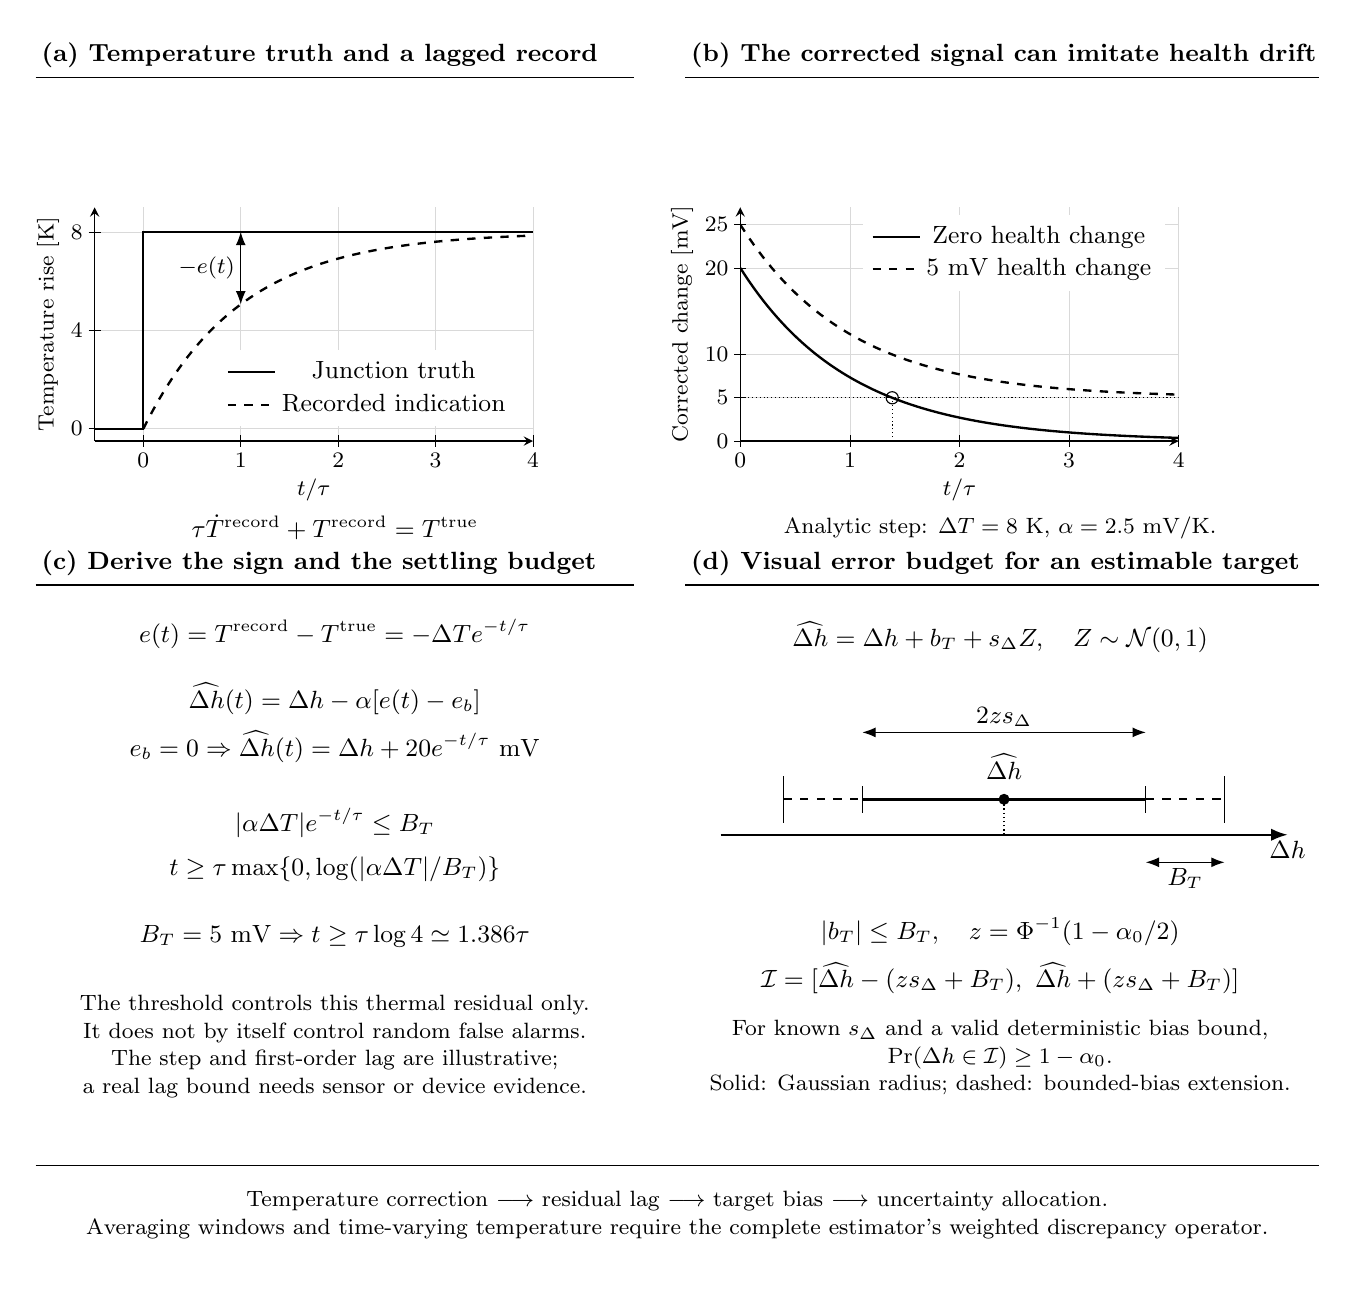
\begin{tikzpicture}[x=1cm,y=1cm]\path[use as bounding box] (0,0) rectangle (16.6,15.8);
\node[head] at (0.1,15.45){(a) Temperature truth and a lagged record};\draw[wire] (0.1,15.17)--(7.699999999999999,15.17);
\node[head] at (8.35,15.45){(b) The corrected signal can imitate health drift};\draw[wire] (8.35,15.17)--(16.4,15.17);
\begin{axis}[mathaxis,at={(.85cm,10.55cm)},anchor=south west,width=7.15cm,height=4.55cm,
 xmin=-.5,xmax=4,ymin=-.5,ymax=9,xtick={0,1,2,3,4},ytick={0,4,8},xlabel={$t/\tau$},ylabel={Temperature rise [K]},
 legend style={at={(.97,.06)},anchor=south east}]
\addplot[line width=.85pt] coordinates {(-.5,0)(0,0)(0,8)(4,8)};\addlegendentry{Junction truth}
\addplot[dashed,domain=0:4,samples=100,line width=.85pt]{8*(1-exp(-x))};\addlegendentry{Recorded indication}
\draw[<->] (axis cs:1,5.056964)--(axis cs:1,8) node[midway,left,tinytext] {$-e(t)$};\end{axis}
\node[eq] at (3.9,9.45){$\tau\dot T^{\mathrm{record}}+T^{\mathrm{record}}=T^{\mathrm{true}}$};
\begin{axis}[mathaxis,at={(9.05cm,10.55cm)},anchor=south west,width=7.15cm,height=4.55cm,
 xmin=0,xmax=4,ymin=0,ymax=27,xtick={0,1,2,3,4},ytick={0,5,10,20,25},xlabel={$t/\tau$},ylabel={Corrected change [mV]},
 legend style={at={(.97,.97)},anchor=north east}]
\addplot[domain=0:4,samples=100,line width=.85pt]{20*exp(-x)};\addlegendentry{Zero health change}
\addplot[domain=0:4,samples=100,dashed,line width=.85pt]{5+20*exp(-x)};\addlegendentry{5 mV health change}
\addplot[domain=0:4,samples=2,densely dotted,forget plot]{5};
\draw[densely dotted] (axis cs:1.386294,0)--(axis cs:1.386294,5);
\addplot[only marks,mark=o,mark size=2.2pt,forget plot] coordinates {(1.386294,5)};\end{axis}
\node[tinytext,align=center] at (12.35,9.45){Analytic step: $\Delta T=8$ K, $\alpha=2.5$ mV/K.};
\node[head] at (0.1,9.0){(c) Derive the sign and the settling budget};\draw[wire] (0.1,8.72)--(7.699999999999999,8.72);
\node[head] at (8.35,9.0){(d) Visual error budget for an estimable target};\draw[wire] (8.35,8.72)--(16.4,8.72);
\node[eq] at (3.9,8.1){$e(t)=T^{\mathrm{record}}-T^{\mathrm{true}}=-\Delta T e^{-t/\tau}$};
\node[eq] at (3.9,6.97){$\widehat{\Delta h}(t)=\Delta h-\alpha[e(t)-e_b]$\\[5pt]
$e_b=0\Rightarrow\widehat{\Delta h}(t)=\Delta h+20e^{-t/\tau}\ \mathrm{mV}$};
\node[eq] at (3.9,5.42){$|\alpha\Delta T|e^{-t/\tau}\leq B_T$\\[5pt]
$t\geq\tau\max\{0,\log(|\alpha\Delta T|/B_T)\}$};
\node[eq] at (3.9,4.26){$B_T=5\ \mathrm{mV}\Rightarrow t\geq\tau\log4\simeq1.386\tau$};
\node[tinytext,align=center] at (3.9,2.86){The threshold controls this thermal residual only.\\It does not by itself control random false alarms.\\The step and first-order lag are illustrative;\\a real lag bound needs sensor or device evidence.};
\draw[arr] (8.8,5.55)--(16.0,5.55) node[below] {$\Delta h$};
\draw[densely dotted,wire] (12.4,5.55)--(12.4,6.0);
\draw[line width=1.2pt] (10.6,6.0)--(14.2,6.0);
\draw[wire] (10.6,5.83)--(10.6,6.17);\draw[wire] (14.2,5.83)--(14.2,6.17);
\fill (12.4,6) circle(2pt);\node[above] at (12.4,6.18){$\widehat{\Delta h}$};
\draw[<->] (10.6,6.85)--(14.2,6.85) node[midway,above] {$2zs_\Delta$};
\draw[dashed,line width=.8pt] (9.6,6)--(10.6,6);\draw[dashed,line width=.8pt] (14.2,6)--(15.2,6);
\draw[wire] (9.6,5.7)--(9.6,6.3);\draw[wire] (15.2,5.7)--(15.2,6.3);
\draw[<->] (14.2,5.2)--(15.2,5.2) node[midway,below] {$B_T$};
\node[eq] at (12.35,8.06){$\widehat{\Delta h}=\Delta h+b_T+s_\Delta Z,\quad Z\sim\mathcal N(0,1)$};
\node[eq] at (12.35,4.01){$|b_T|\leq B_T,\quad z=\Phi^{-1}(1-\alpha_0/2)$\\[5pt]
$\mathcal I=[\widehat{\Delta h}-(zs_\Delta+B_T),\ \widehat{\Delta h}+(zs_\Delta+B_T)]$};
\node[tinytext,align=center] at (12.35,2.72){For known $s_\Delta$ and a valid deterministic bias bound,\\$\Pr(\Delta h\in\mathcal I)\geq1-\alpha_0$.\\Solid: Gaussian radius; dashed: bounded-bias extension.};
\draw[wire] (.1,1.35)--(16.4,1.35);
\node[tinytext,align=center] at (8.25,.72){Temperature correction $\longrightarrow$ residual lag $\longrightarrow$ target bias $\longrightarrow$ uncertainty allocation.\\Averaging windows and time-varying temperature require the complete estimator's weighted discrepancy operator.};
\end{tikzpicture}
\PlateCaption{\textbf{Figure 9.} Pointwise analytic illustration, without noisy samples or simulated sensor evidence. The baseline is settled and the junction temperature undergoes a step; the indication follows a first-order lag. Curves compare zero health change and a true 5 mV change. The interval in (d) adds a deterministic bias budget to Gaussian uncertainty; it is valid only for an estimable target, correct variance, and a justified bound. It is not an inferred uncertainty statement for the retained SIL trials.}

\newpage
\PlateTitle{10}{From one calibrated decision to a complete monitoring task}
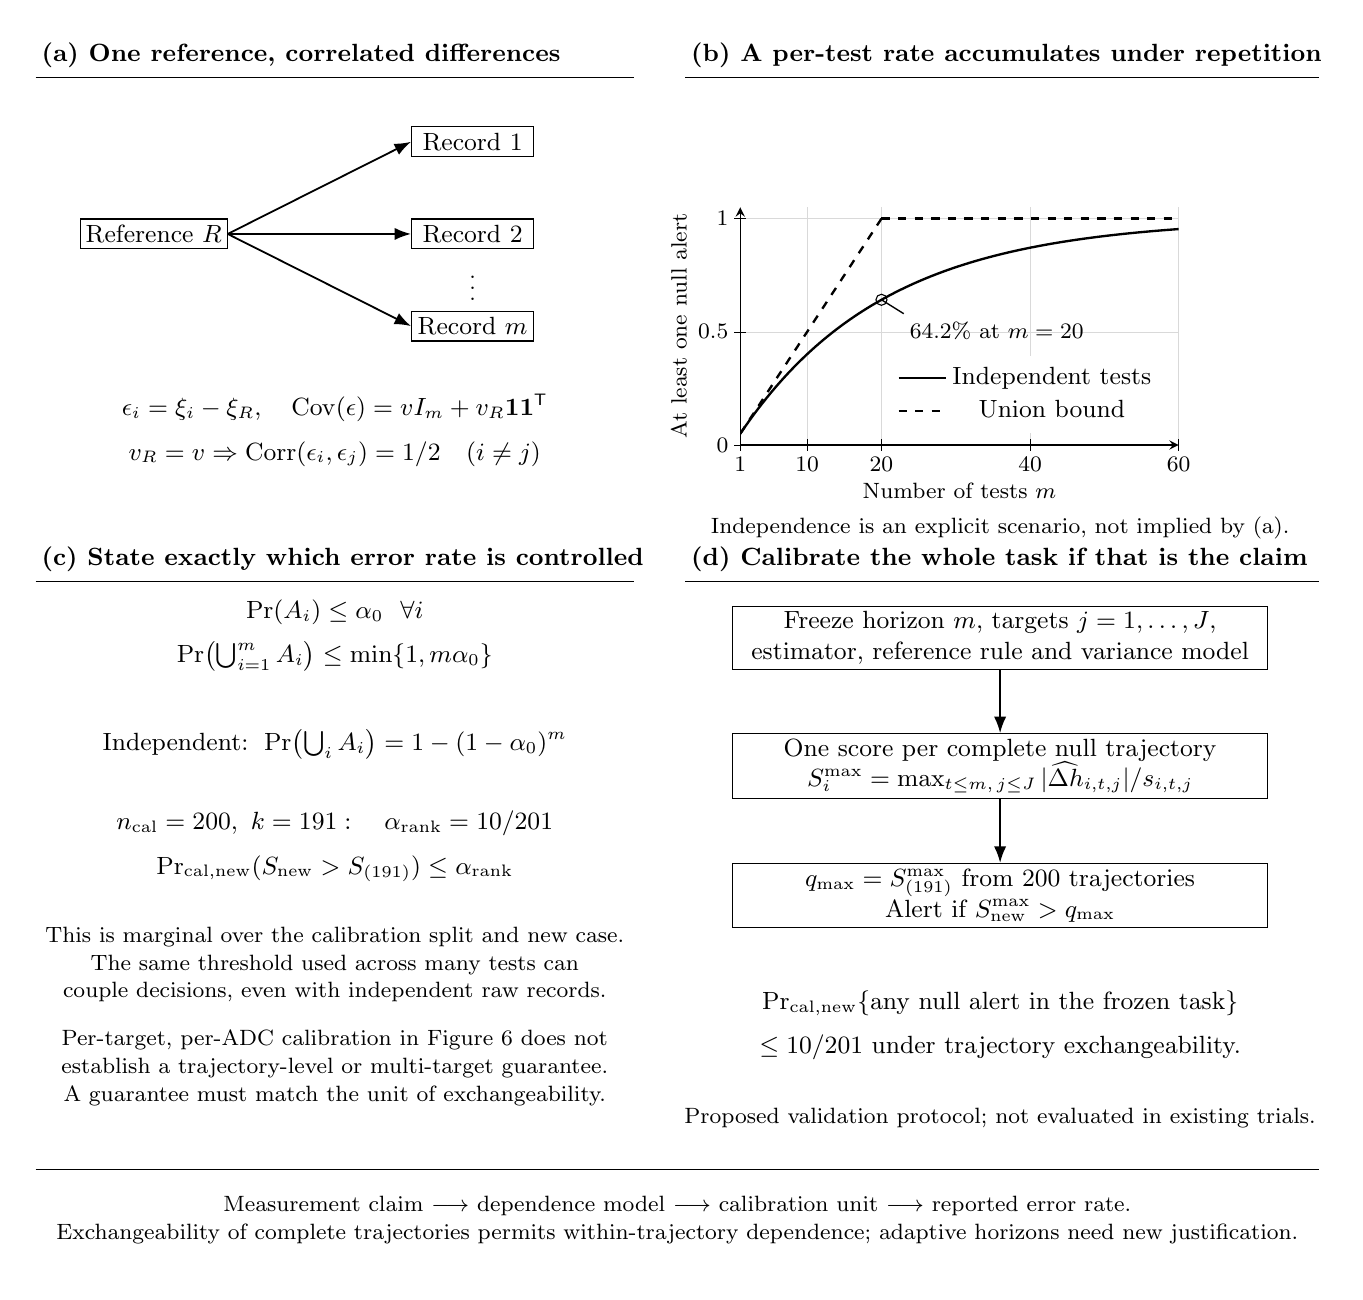
\begin{tikzpicture}[x=1cm,y=1cm]\path[use as bounding box] (0,0) rectangle (16.6,15.8);
\node[head] at (0.1,15.45){(a) One reference, correlated differences};\draw[wire] (0.1,15.17)--(7.699999999999999,15.17);
\node[head] at (8.35,15.45){(b) A per-test rate accumulates under repetition};\draw[wire] (8.35,15.17)--(16.4,15.17);
\node[device,minimum width=1.75cm] (ref) at (1.6,13.18){Reference $R$};
\node[device,minimum width=1.55cm] (m1) at (5.65,14.35){Record 1};
\node[device,minimum width=1.55cm] (m2) at (5.65,13.18){Record 2};
\node[device,minimum width=1.55cm] (mm) at (5.65,12.01){Record $m$};
\draw[arr] (ref.east)--(m1.west);\draw[arr] (ref.east)--(m2.west);\draw[arr] (ref.east)--(mm.west);
\node[tinytext] at (5.65,12.6){$\vdots$};
\node[eq] at (3.9,10.69){$\epsilon_i=\xi_i-\xi_R,\quad\Cov(\epsilon)=vI_m+v_R\one\one\trans$\\[5pt]
$v_R=v\Rightarrow\operatorname{Corr}(\epsilon_i,\epsilon_j)=1/2\quad(i\neq j)$};
\begin{axis}[mathaxis,at={(9.05cm,10.5cm)},anchor=south west,width=7.15cm,height=4.6cm,
 xmin=1,xmax=60,ymin=0,ymax=1.05,xtick={1,10,20,40,60},ytick={0,.5,1},xlabel={Number of tests $m$},ylabel={At least one null alert},
 legend style={at={(.97,.05)},anchor=south east}]
\addplot[domain=1:60,samples=100,line width=.85pt]{1-.95^x};\addlegendentry{Independent tests}
\addplot[domain=1:20,samples=40,dashed,line width=.85pt]{.05*x};
\addplot[domain=20:60,samples=2,dashed,line width=.85pt,forget plot]{1};\addlegendentry{Union bound}
\addplot[only marks,mark=o,mark size=2pt,forget plot] coordinates {(20,.641514)};
\draw[wire] (axis cs:20,.641514)--(axis cs:23,.58);
\node[tinytext,anchor=north west] at (axis cs:23,.57){$64.2\%$ at $m=20$};\end{axis}
\node[tinytext,align=center] at (12.35,9.45){Independence is an explicit scenario, not implied by (a).};
\node[head] at (0.1,9.05){(c) State exactly which error rate is controlled};\draw[wire] (0.1,8.770000000000001)--(7.699999999999999,8.770000000000001);
\node[head] at (8.35,9.05){(d) Calibrate the whole task if that is the claim};\draw[wire] (8.35,8.770000000000001)--(16.4,8.770000000000001);
\node[eq] at (3.9,8.08){$\Pr(A_i)\leq\alpha_0\ \ \forall i$\\[5pt]
$\Pr\!\left(\bigcup_{i=1}^m A_i\right)\leq\min\{1,m\alpha_0\}$};
\node[eq] at (3.9,6.7){$\text{Independent: }\Pr\!\left(\bigcup_i A_i\right)=1-(1-\alpha_0)^m$};
\node[eq] at (3.9,5.4){$n_{\mathrm{cal}}=200,\ k=191:\quad\alpha_{\mathrm{rank}}=10/201$\\[5pt]
$\Pr_{\mathrm{cal,new}}(S_{\mathrm{new}}>S_{(191)})\leq\alpha_{\mathrm{rank}}$};
\node[tinytext,align=center] at (3.9,3.9){This is marginal over the calibration split and new case.\\The same threshold used across many tests can\\couple decisions, even with independent raw records.};
\node[tinytext,align=center] at (3.9,2.59){Per-target, per-ADC calibration in Figure 6 does not\\establish a trajectory-level or multi-target guarantee.\\A guarantee must match the unit of exchangeability.};
\node[draw,align=center,minimum width=6.8cm] (traj) at (12.35,8.05){Freeze horizon $m$, targets $j=1,\ldots,J$,\\estimator, reference rule and variance model};
\node[draw,align=center,minimum width=6.8cm] (score) at (12.35,6.42){One score per complete null trajectory\\$S_i^{\max}=\max_{t\leq m,\,j\leq J}|\widehat{\Delta h}_{i,t,j}|/s_{i,t,j}$};
\node[draw,align=center,minimum width=6.8cm] (quant) at (12.35,4.78){$q_{\max}=S_{(191)}^{\max}$ from 200 trajectories\\Alert if $S_{\mathrm{new}}^{\max}>q_{\max}$};
\draw[arr] (traj.south)--(score.north);\draw[arr] (score.south)--(quant.north);
\node[eq] at (12.35,3.13){$\Pr_{\mathrm{cal,new}}\{\text{any null alert in the frozen task}\}$\\[5pt]
$\leq10/201$ under trajectory exchangeability.};
\node[tinytext,align=center] at (12.35,1.95){Proposed validation protocol; not evaluated in existing trials.};
\draw[wire] (.1,1.3)--(16.4,1.3);
\node[tinytext,align=center] at (8.25,.66){Measurement claim $\longrightarrow$ dependence model $\longrightarrow$ calibration unit $\longrightarrow$ reported error rate.\\Exchangeability of complete trajectories permits within-trajectory dependence; adaptive horizons need new justification.};
\end{tikzpicture}
\PlateCaption{\textbf{Figure 10.} Reference reuse gives an explicit dependence mechanism. Panel (b) shows the exact independent-test familywise rate at $\alpha_0=0.05$ alongside the dependence-agnostic union bound, rather than observed alarm data. Panel (d) is a proposed finite-horizon calibration protocol: exchangeable complete null trajectories are its sampling units. Its rank guarantee is marginal and requires the entire task to be frozen before calibration. Existing per-target SIL rates are retained as narrower evidence.}

\end{document}
